\documentclass[english]{panikzettel}

\usepackage{cleveref}
\usepackage{todonotes}
\usepackage{listings,lstautogobble}
\lstset{
	language=C,
	tabsize=4,
	basicstyle=\ttfamily,
	autogobble=true,
	breaklines=true
}

\usepackage{float}
\usepackage{graphicx}

\usepackage{fontspec}
\setmonofont[
  Contextuals=Alternate,
	Scale=MatchLowercase
	]{FiraCode Nerd Font}

\newcommand{\fkt}[1]{\texttt{#1}(\(\cdot\))}
\newcommand{\alert}[1]{\textbf{\textcolor{red!75!black}{#1}}}

\title{Communications Systems Engineering}
\author{Moritz Hüllmann}

\begin{document}
	\pagenumbering{gobble}
	\maketitle
	\setcounter{tocdepth}{2}
	\tableofcontents

	\newpage
	\pagenumbering{arabic}
	\section{Introduction}
	\label{s-introduction}
	
	A \textit{Communication System} is a system, that provides functionality in order to be able to transmit data to other communicating parties.

	\textit{Communication Services} implement concrete components with standardized interfaces, upon which communication systems are build.

	A \textit{Protocol} combines all those components into one entity.
	They define \textit{messages} in a specific \textit{format}, which obey \textit{rules} for sending and receiving data.
	Protocols can be implemented on all layers of the ISO/OSI reference model, except layer 1 and 2, as they are responsible for the physical transportation of bits.

	\begin{figure}[H]
		\centering
		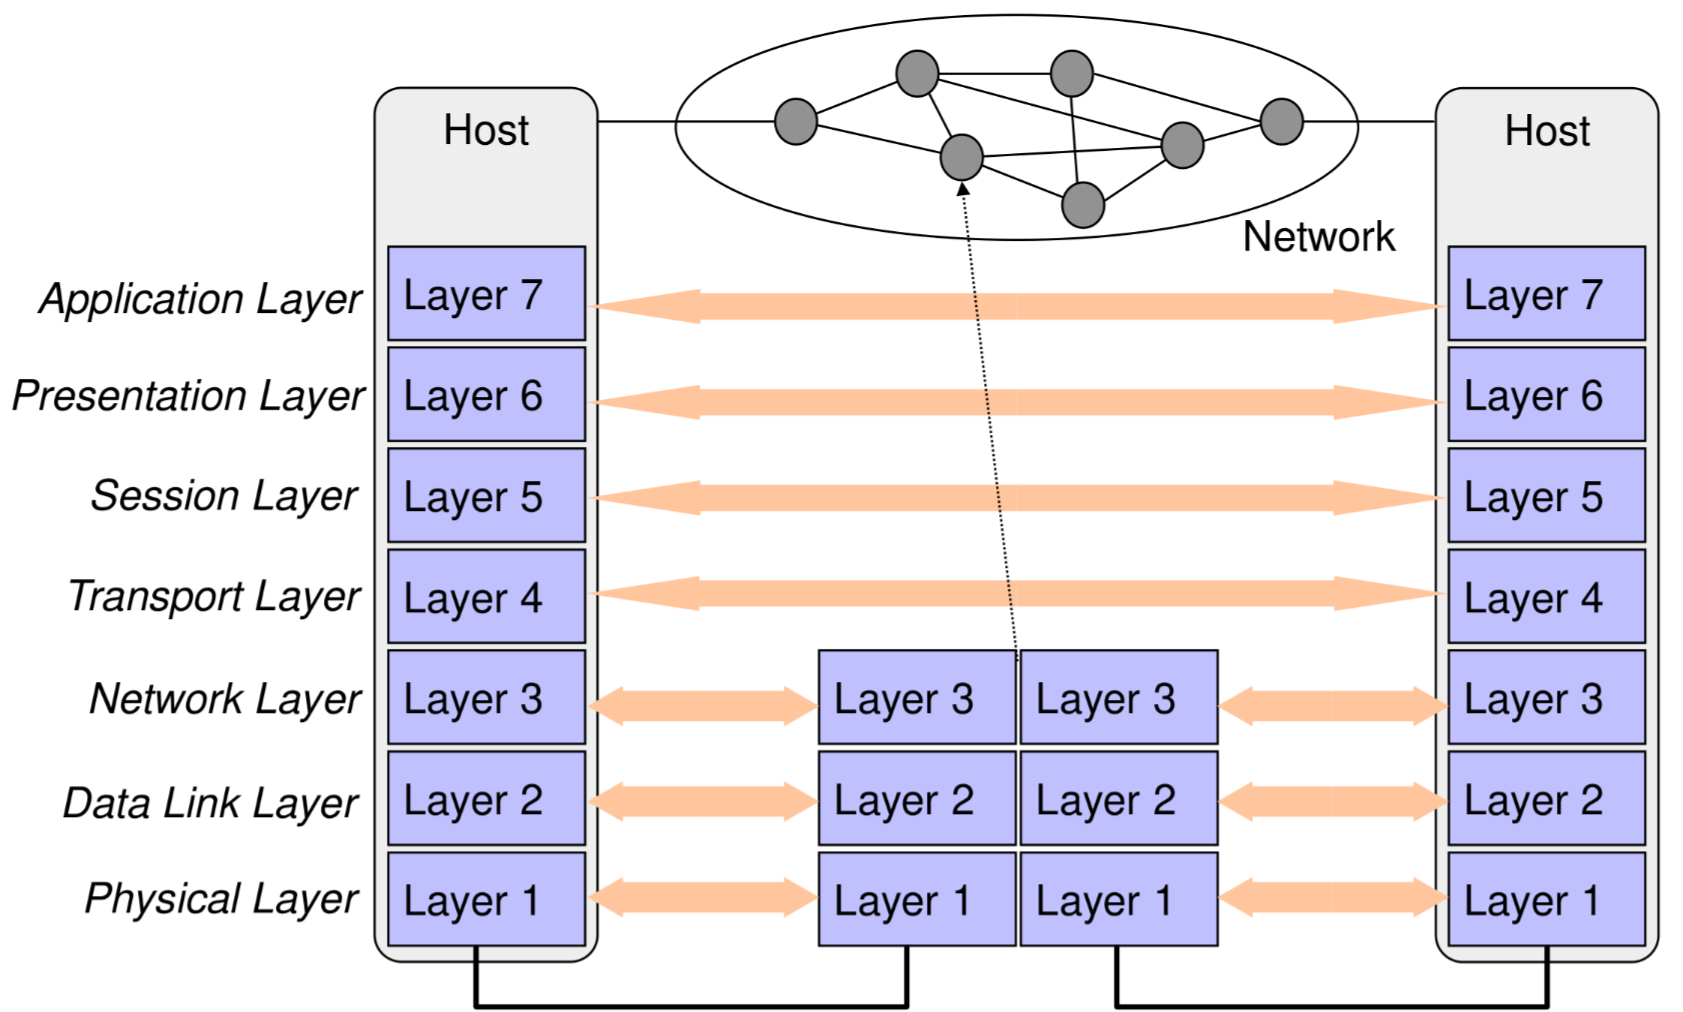
\includegraphics[width=\textwidth]{img/0-iso-osi.png}
		\caption{ISO/OSI}
		\label{img-0-iso-osi}
	\end{figure}
	
	Units of communication are called \textit{Packets}, which are structured, within the linux kernel, as shown in the following.

	\begin{figure}[H]
		\centering
		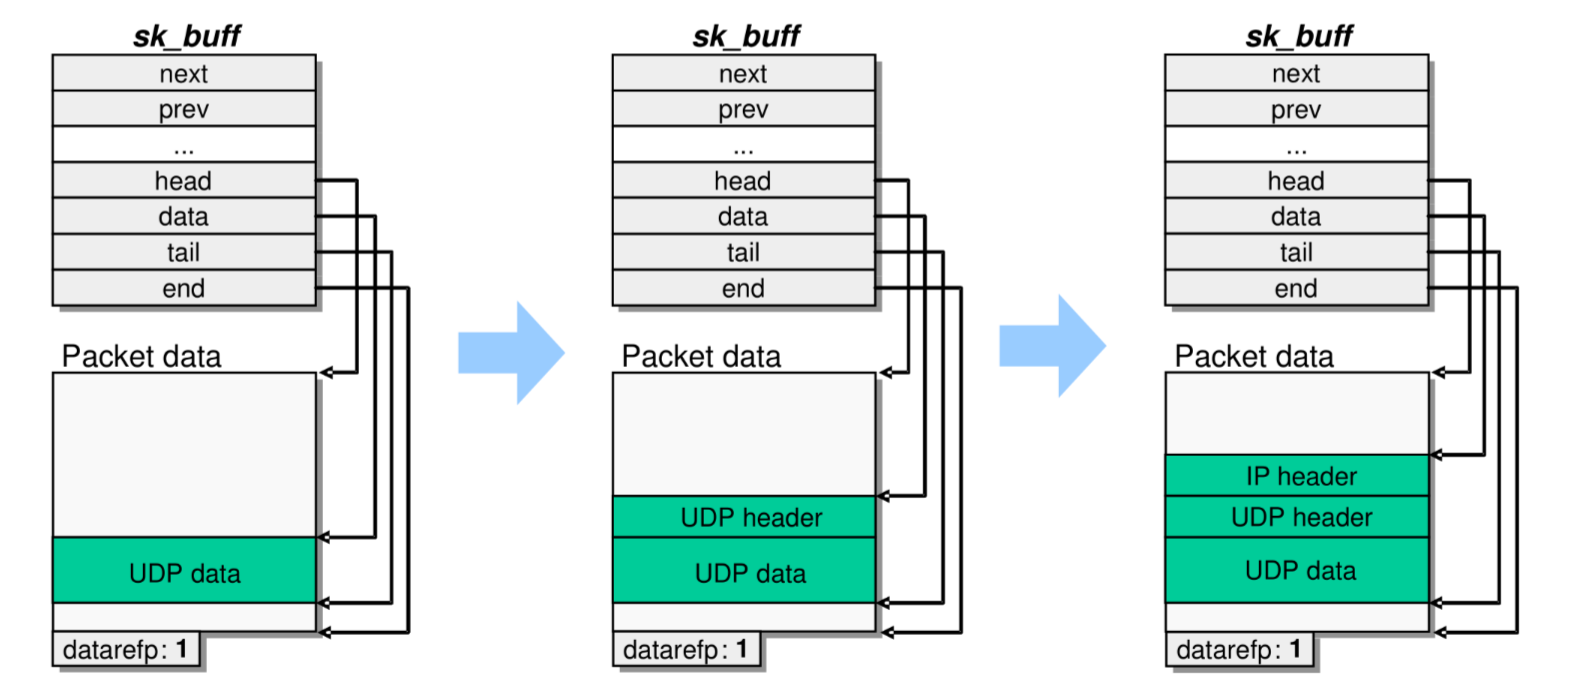
\includegraphics[width=\textwidth]{img/0-paket-kernel-rep.png}
		\caption{Packets in the Linux kernel}
		\label{img-0-paket-kernel-rep}
	\end{figure}
	
	Each layer simply adds its header to the structure, thus minimizing copy-operations.

	\subsection{Clayton Tunnel Protocol}
	\label{ss-clayton-tunnel-protocol}
	\begin{halfboxl}
		This particular malformed protocol was meant to ensure, that only one train enters a tunnel per track. 
		
		However, the protocol was not suited for signalling, that more than one train is in the tunnel, which leads to \textit{Undefined Behavior} in cases where this happens on accident.
	\end{halfboxl}
	\begin{halfboxr}
		\vspace{-\baselineskip}
		\begin{figure}[H]
			\centering
			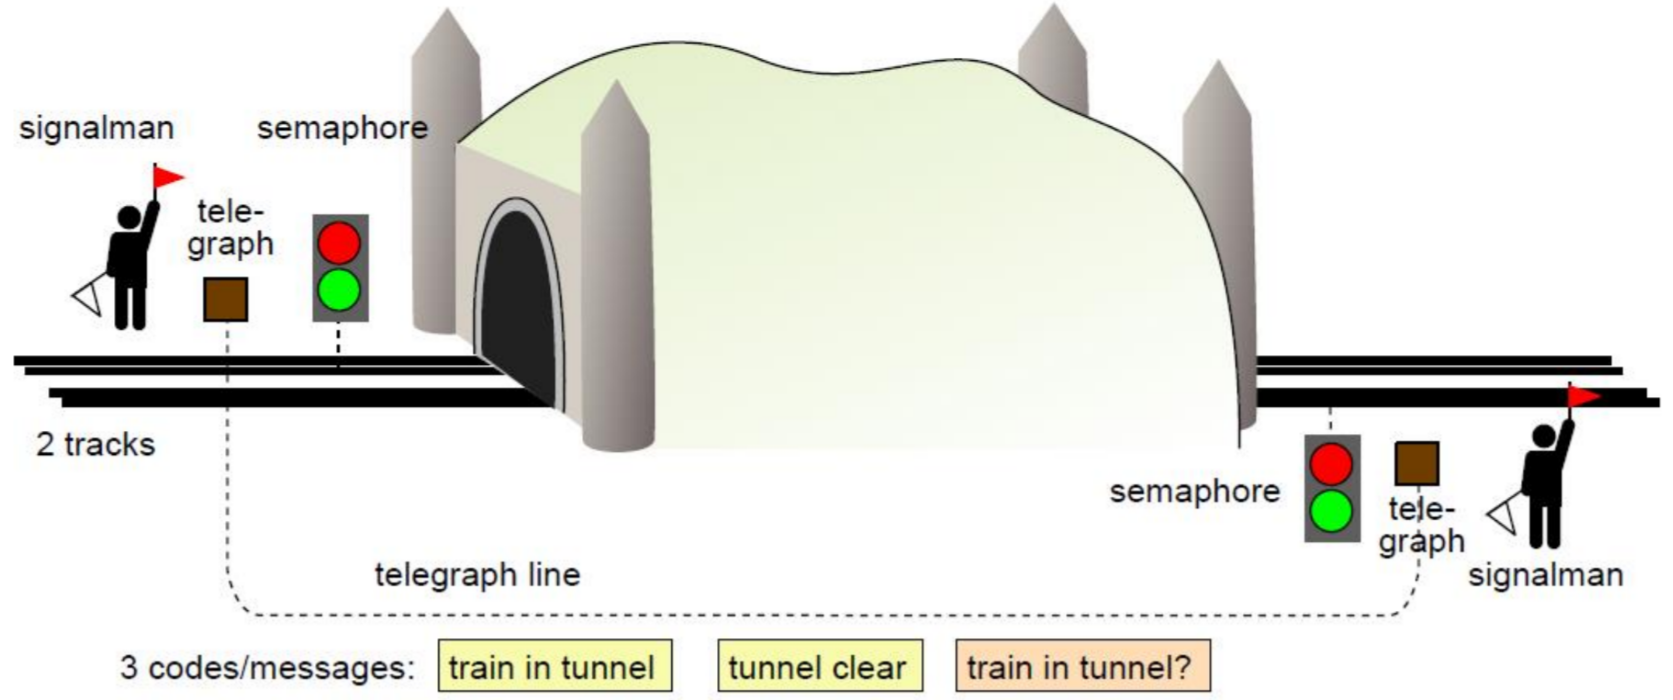
\includegraphics[width=\textwidth]{img/0-clayton.png}
			\caption{Depiction of the Clayton Tunnel Protocol}
			\label{img-0-clayton}
		\end{figure}
	\end{halfboxr}
	
	\newpage
	\section{Network Programming}

	There are five socket types, but only three are relevant.
	\begin{itemize}
		\item \texttt{SOCK\_RAW}
		\item \texttt{SOCK\_STREAM}
		\item \texttt{SOCK\_DGRAM}
		\item \texttt{SOCK\_RDM}
		\item \texttt{SOCK\_SEQPACKET}
	\end{itemize}
	Combined with \textbf{Protocol Family}, communication is defined completely.
	Focus is on \textbf{IPv4/v6}.
	Relevant protocol families
	\begin{itemize}
		\item \texttt{PF\_INET} – IPv4
		\item \texttt{PF\_INET6} – IPv6
	\end{itemize}
	Sockets give access to \textbf{transport layer}.
	One may also use \texttt{AF} instead of \texttt{PF} prefixes.
	
	\subsection{C-Implemenation of Sockets}

	\begin{defi}{\fkt{socket}}
		This function creates a new reference to a socket in the OS.
		\begin{lstlisting}[language=C]
			int socket(int socket_family, int socket_type, int protocol);
		\end{lstlisting}
		\tcblower
		\texttt{protocol} – optional, if there is only one possibility. 
		Set to \texttt{0} if not wanted

		\textbf{Returns:} 0 on success, -1 on error
	\end{defi}

	\begin{defi}{\fkt{bind}}
		This socket binds a socket to a specific address and port.
		\begin{lstlisting}[language=C]
			int bind(int sock, const struct sockaddr* addr, socklen_t addrlen);
		\end{lstlisting}
		\tcblower
		\texttt{sock} – a file descriptor, i.e. the return value of \fkt{socket}

		\textbf{Returns:} 0 on success, -1 on error
	\end{defi}
	\fkt{bind} – commonly used by servers.
	\texttt{strcut sockaddr* addr} has all information regarding IPv4/v6.

	One has to be careful regarding byte order. 
	Sockets usualy require \textbf{network byte order}. 
	
	\begin{description}
		\item[\fkt{htonl}] Host to network long
		\item[\fkt{ntohl}] Network to host long
		\item[\dots] and many more
	\end{description}

	\begin{defi}{\fkt{getaddrinfo}}
		This function gets all possible based on the information passed to it.
		Can be used to determine IP addresses, ports and so on.
		\begin{lstlisting}[language=C]
			int getaddrinfo(const char *node, const char *service, const struct addrinfo *hints, struct addrinfo **res);	
		\end{lstlisting}
		\tcblower
		\texttt{hints} – used to tell the function what is should do specifically.

		\textbf{Returns:} 0 on success, -1 on error. 
		On success, \texttt{res} contains a pointer to a linked list of whatever was requested
	\end{defi}
	This function should be used everytime, one implements server/client applications, as it can handle DNS resolution, handle both IPv4 and v6 and so on.

	Suggested call order:
	\begin{enumerate}
		\item \fkt{getaddrinfo}
		\item \fkt{socket}
		\item \fkt{bind}
	\end{enumerate}

	\begin{figure}[H]
		\centering
		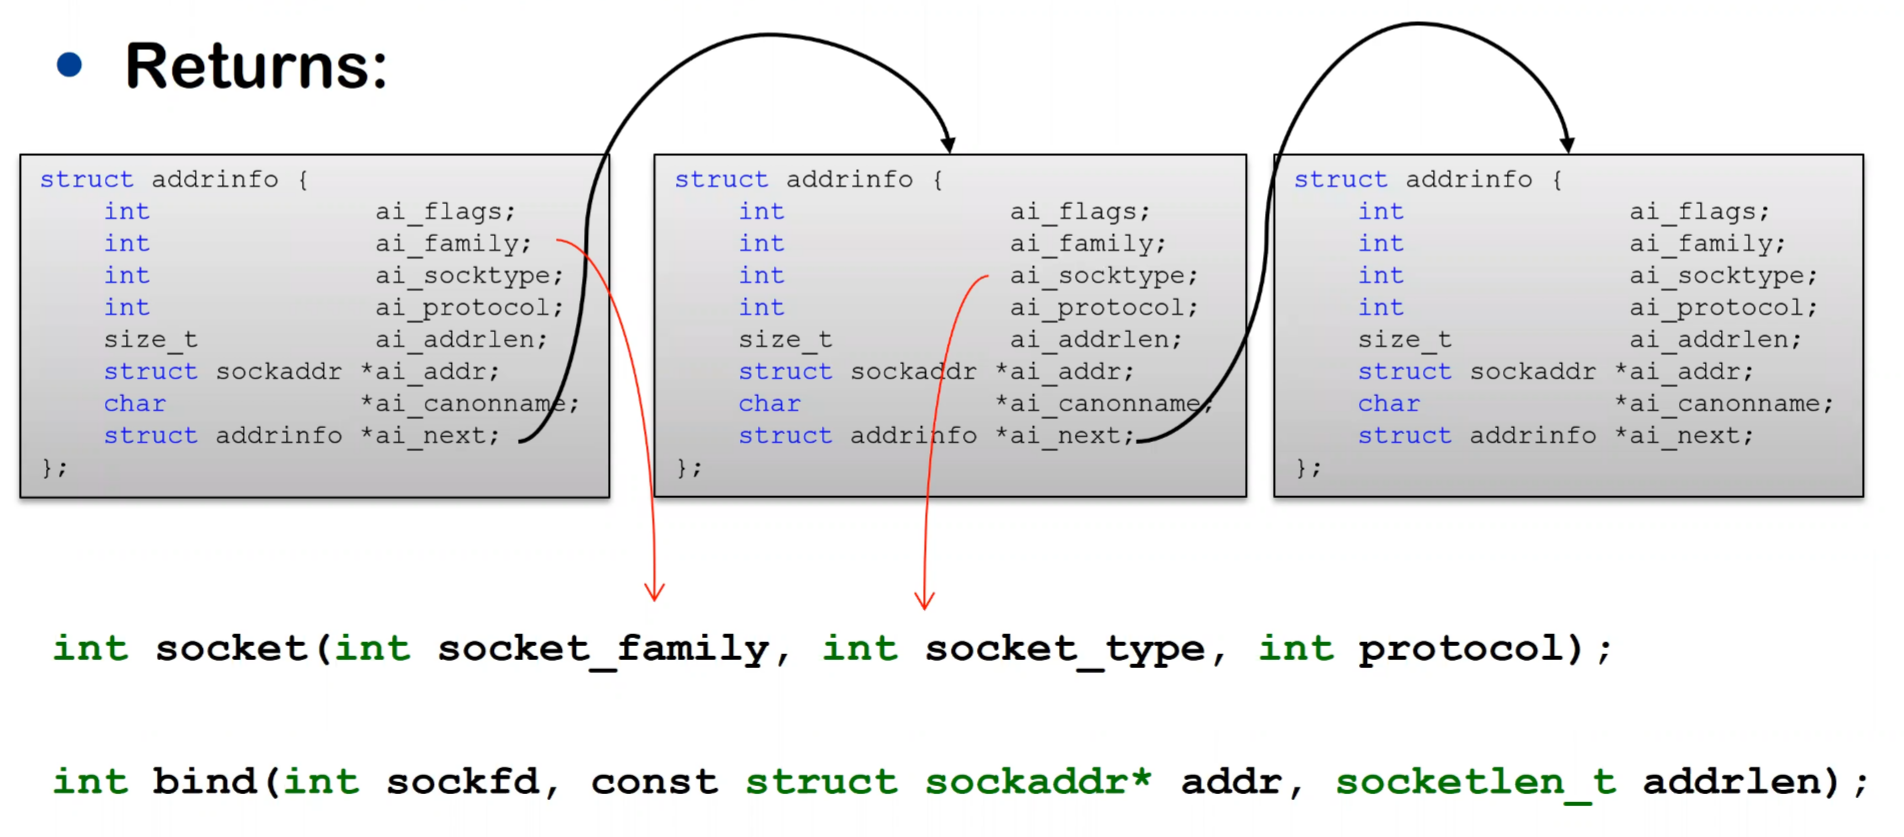
\includegraphics[width=\textwidth]{img/1-getaddrinfo-usage.png}
		\caption{How to use \fkt{getaddrinfo}. Note: All information used should originate in one block, not two as shown above.}
		\label{img-1-getaddrinfo-usage}
	\end{figure}	
	
	\subsubsection{Server-side Programming}

	Up until now, only communication setup was discussed, we need to communicate now.

	\begin{defi}{\fkt{listen}}
		This functions listens for incoming connection requests.
		\begin{lstlisting}[language=C]
				int listen(int sockfd, int backlog);
		\end{lstlisting}
		\tcblower
		\texttt{sockfd} – Socket to listen on.	
		
		\texttt{backlog} – Queue length for pending requests.
	
		\textbf{Note:} This is only valid with \texttt{SOCK\_STREAM} and \texttt{SOCK\_SEQPACKET}.
	\end{defi}
	If the queue is full, the server will not answer.
	\fkt{listen} is a blocking function.

	\begin{defi}{\fkt{accept}}
		This function is used to accept requests received by \fkt{listen}.
		\begin{lstlisting}[language=C]
			int accept(int sockfd, struct sockaddr *addr, socklen_t *addrlen);
		\end{lstlisting}
		\tcblower
		\texttt{addr} – holds the address that should be accepted
		
		\texttt{addrlen} – length of \texttt{addr}. One can pass a structure that is big enough for IPv4 and IPv6.

		\textbf{Returns:} File descriptor for new socket, that handles the accepted connection from now on.
	\end{defi}

	\subsubsection{Client-side Programming}

	\begin{defi}{\fkt{connect}}
		This function connects the socket to a server.
		It may perform a TCP handshake and similar things in the process.
		\begin{lstlisting}[language=C]
			int connect(int sockfd, struct sockaddr *addr, socklen_t addrlen);
		\end{lstlisting}
		\tcblower
		\texttt{addr} – address to connect to

		\texttt{addrlen} – length of the address

		\textbf{Returns:} 0 on success, -1 on failure
	\end{defi}
	
	\subsubsection{Sending and Receiving}
	
	One can \textit{write} to and \textit{read} from sockets, with the following functions:
	\begin{itemize}
		\item \fkt{write} and \fkt{read}
		\item \fkt{send} and \fkt{recv} – TCP
		\item \fkt{sendto} and \fkt{recvfrom} – UDP
	\end{itemize}
	
	\begin{defi}{Stream}
		A stream is like reading from a file. TCP just decides to cut the stream at certain points and transmits each fragments as packets.
		We do not know the context of a single packet.
	\end{defi}

	\begin{defi}{Datagram}
		Messages transmitted via datagrams are not cut up by the kernel, they are send as is. If the message is too large, there either is an error, or the package gets fragmented. 
		Each datagram is self-contained, so every received packet can be seen as a unit. 
 	\end{defi}

	\begin{defi}{\fkt{send}/\fkt{write}}
		These functions can be used to write to a socket. 
		As in Linux everything is a file, one can use \fkt{write} instead of \fkt{send}.
		\begin{lstlisting}[language=C]
			ssize_t send(int sockfd, const void* buf, size_t len, int flags);
			ssize_t write(int fd, const void* buf, size_t count);
		\end{lstlisting}
		\tcblower
		\texttt{flags} – instruct kernel to handle send request in a certain way

		\texttt{buf} – Buffer with data to send

		\textbf{Returns:} Bytes actually written. -1 on error, non-negative otherwise 
		\textbf{Note:} \fkt{write} is equals to \fkt{send} with \( \texttt{flags} = 0\)
	\end{defi}

	\begin{defi}{\fkt{recv}/\fkt{read}}
		These functions are designed to read a certain amount of bytes from a socket (or file).
		\begin{lstlisting}[language=C]
			ssize_t recv(int sockfd, void* buf, size_t len, int flags);
			ssize_t read(int fd, void* buf, size_t count);
		\end{lstlisting}
		\tcblower
		Parameters are analogous to \fkt{send}.
	\end{defi}
	Actually using the return value of the reading functions is really important.
	It may be unknown, how many bytes the applications is going to receive in a single read operation.
	If \( retval \not= lenght \), then not enough was read. 

	\begin{defi}{\fkt{sendto} for connection-less sockets}
		This function sends a certain amount of bytes from a buffer to the specified address and port.
		\begin{lstlisting}[language=C]
			ssize_t sendto(int sockfd, const void* buf, size_t len, int flags, const struct sockaddr *dest_addr, socklen_t addrlen);
		\end{lstlisting}
		\tcblower
		\texttt{dest\_addr} – Address and port to send to 

		\textbf{Note:} There is no equivalent \texttt{write} function.
		
		\textbf{Note:} Parameters up to \texttt{flags} same as for \fkt{send}. 
		Exclusively for sending datagrams.
	\end{defi}

	\begin{defi}{\fkt{recvfrom} for connection-less sockets}
		This functions receives a certain amount of bytes from a given address.
		\begin{lstlisting}[language=C]
			ssize_t recvfrom(int sockfd, void* buf, size_t len, int flags, const struct sockaddr *src_addr, socklen_t *addrlen);
		\end{lstlisting}
		\tcblower
		\textbf{Note:} \texttt{src\_addr} will be replaced with the address, that really was received from. 
		\texttt{addrlen} will then hold the correct length of the structure.

		\textbf{Note:} Parameters up to \texttt{flags} same as \fkt{recv}.
	\end{defi}

	Again, if it is not known which version of IP is going to be used, use \texttt{struct sockaddr\_storage}, to allow for both versions.

	\subsubsection{Closing Connections}

	There are several methods for closing a connection, each to be used in a different scenario.

	\begin{defi}{\fkt{close}}
		Drops all pakets queued for receiving and sending, and shuts down everything else related to the socket. Also frees all previously allocated space.
		\begin{lstlisting}[language=C]
			int close(int sockfd);
		\end{lstlisting}
		\tcblower
		\textbf{Returns:} 0 on success, -1 on error
	\end{defi}

	For more conservative shutdown operations, the following function can be used.

	\begin{defi}{\fkt{shutdown}}
		More conservative \fkt{close} variant.
		\begin{lstlisting}[language=C]
			int shutdown(int sockfd, int flags);
		\end{lstlisting}
		\tcblower
		\texttt{flags} – 0: no further receives, 1: no further sends, 2: both

		\textbf{Note:} Return values same as for \fkt{close}

		\textbf{Note:} Sends \texttt{FIN} and/or \texttt{FIN\_ACK}, other party might get \texttt{RST} (reset) when trying to read from the shut down socket

		\textbf{Note:} This allows all queued data to be send.
	\end{defi}

	\fkt{shutdown} cannot stand alone. 
	\fkt{close} must be called after a call to \fkt{shutdown}, as it releases all hugged \texttt{struct}s.

	\subsubsection{Connection Overview}

	\begin{figure}[H]
		\centering
		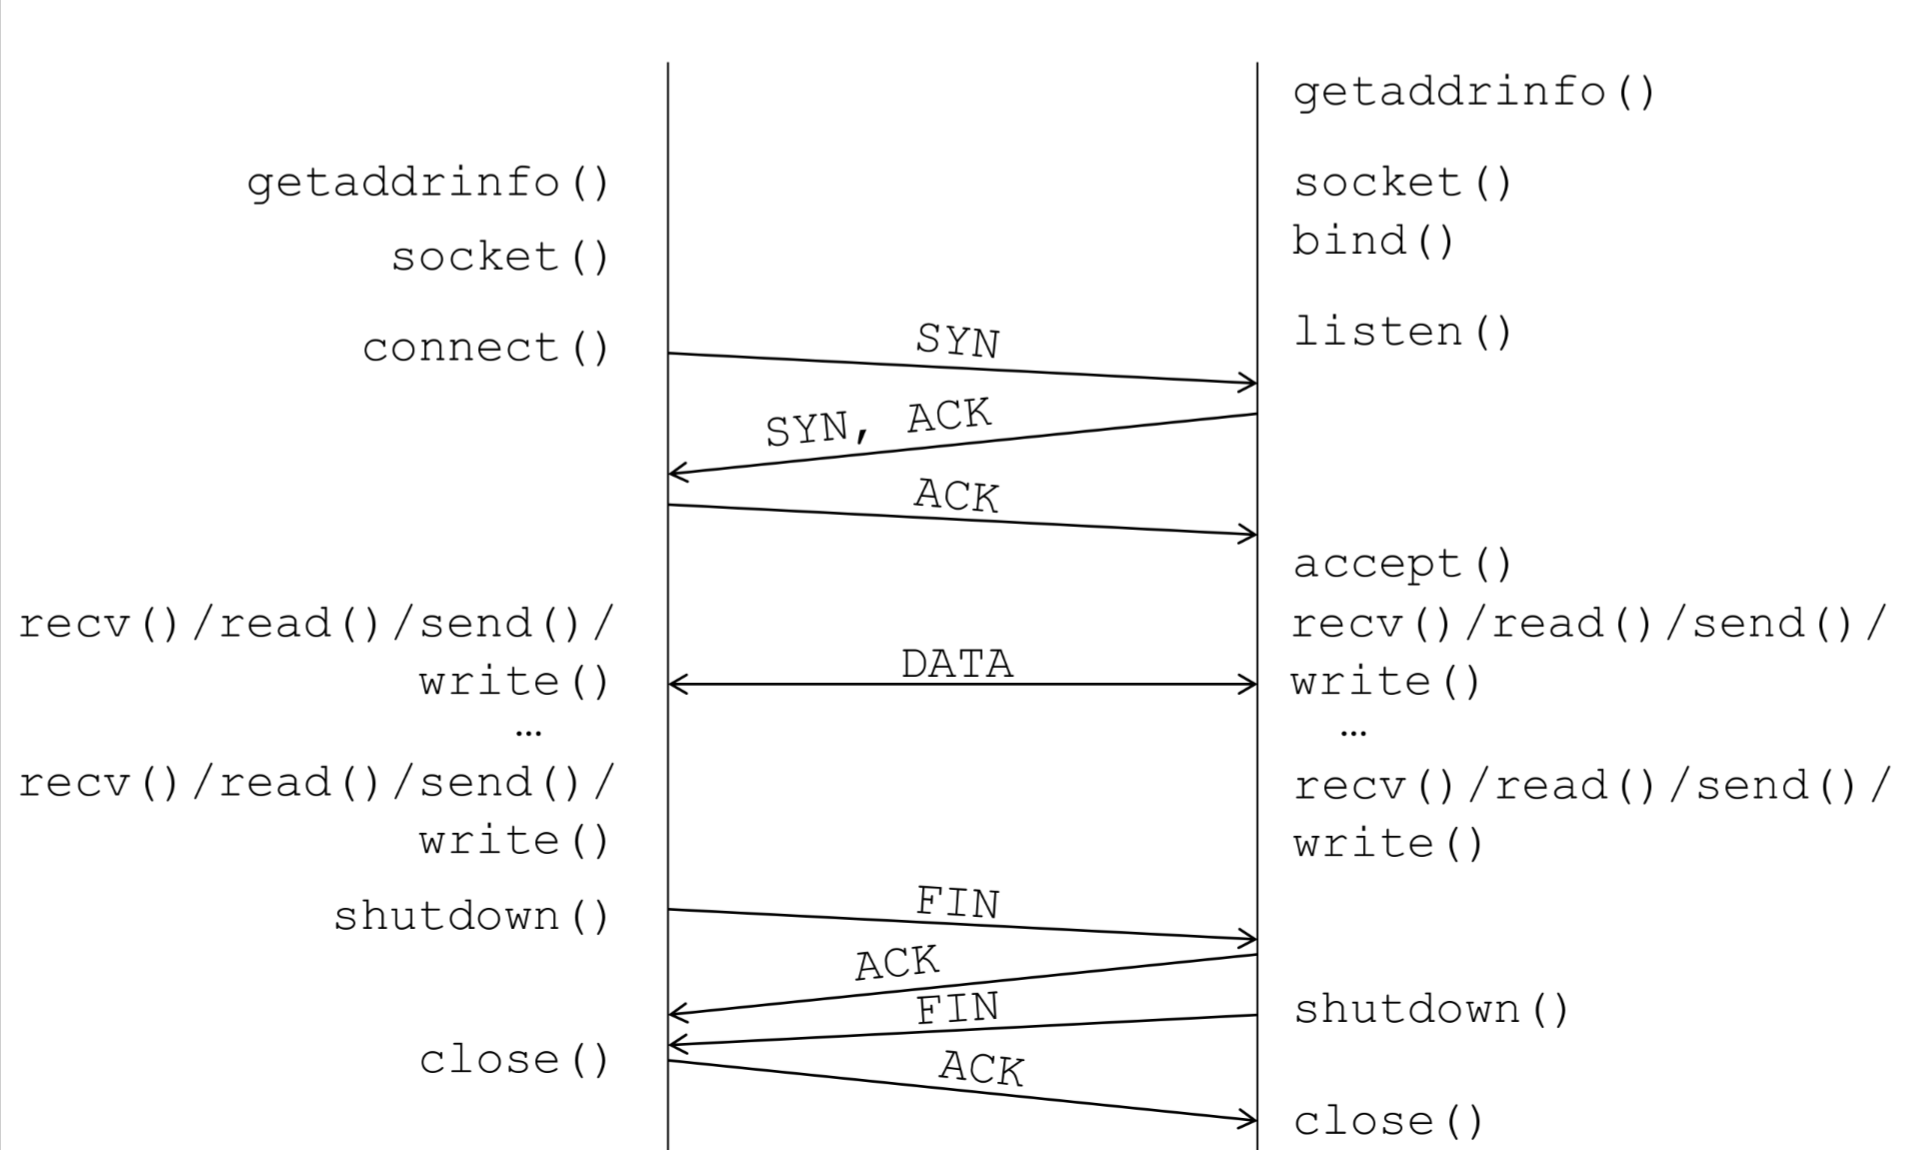
\includegraphics[width=\textwidth]{img/1-connection-overview.png}
		\caption{Overview over the course of a connection-aware socket}
		\label{img-1-connection-overview}
	\end{figure}

	\subsubsection{Configuring a Socket}

	\begin{defi}{\fkt{setsockopt}}
		Apply options to sockets.
		\begin{lstlisting}[language=C]
			int setsockopt(int sockfd, int level, int optname, const void* optval, socklen_t optlen);
		\end{lstlisting}
		\tcblower
		\texttt{level} – basicalli ISO/OSI level the option should be applied to
		
		\textbf{Returns:} 0 on success, -1 on error
	\end{defi}
	
	Getting options set for a sockets uses a functions with more or less the same signature as \fkt{setsockopt}, but is called \texttt{getsockopt}.

	\texttt{I/O}-controls can also be used to set and read properties of a socket. Commonly:
	\begin{itemize}
		\item Timestamp of last received packet
		\item How many bytes are unsend (TCP)
		\item How many bytes are unread (TCP)
		\item \dots
	\end{itemize}
	
	\subsubsection{Non-blocking Sockets}
	
	There are two methods that one could use: \fkt{select} and \texttt{epoll}.

	\paragraph{Non-blocking Sockets using \fkt{select}}
	All network calls are blocking by default. 
	This is not optimal in a server setting, as this introduces great overhead and occupies many ressources of the server, that could be used elsewhere. 
	\textbf{Threads} are not an option for highly scalable systems, as they introduce great computation overhead.
	\fkt{fcntl} can be used to set flags to sockets, specically \texttt{O\_NONBLOCK}.
	Callbacks are called, to notify a program, if a socket is write-/readable.
	Polling is not an option, this is busy waiting.	

	\begin{defi}{\fkt{select}}
		\begin{lstlisting}[language=C]
			int select(int nfds, fd_set *readfds, fd_set *writefds, fd_set *exceptfds, struct timeval *timeout);
		\end{lstlisting}
		\tcblower
		\texttt{nfds} – highest file descriptor number in all sets + 1 
		
		\texttt{readfds} – list of sockets to monitor readability for 

		\texttt{writefds} – list of sockets to monitor writeability for

		\texttt{exceptfds} – list of sockets to monitor exceptions for
		
		\texttt{timeout} – maxium wait time
		
		\textbf{Returns:} 0 on timeout, -1 on error, else number of fd's with event \texttt{read/write/excetpfds} is then set to the sockets with events. Manual checking which sockets have events is required.
		\texttt{}
	\end{defi}

	\paragraph{Non-blocking Sockets using \texttt{epoll}}

	It knows two modes:
	\begin{enumerate}
		\item level triggered, which is just as \fkt{select}
		\item and edge triggered.
	\end{enumerate}

	Edge triggered \texttt{epoll} informs on every \textit{change} of states for read and write queues, as well as excepts. 

	If there are 5 new bytes received, calling \texttt{epoll} returns that new data is readable. 
	However, if just 1 byte is read and \texttt{epoll} called again, it will block, as there is no \textbf{new} data available.

	An \texttt{epoll} file descriptor is attached to the sockets queue, directly in the kernel.
	Each \texttt{epoll} \textit{fd} has a queue of its own, and notifies for every socket listed there.

	\begin{figure}[H]
		\centering
		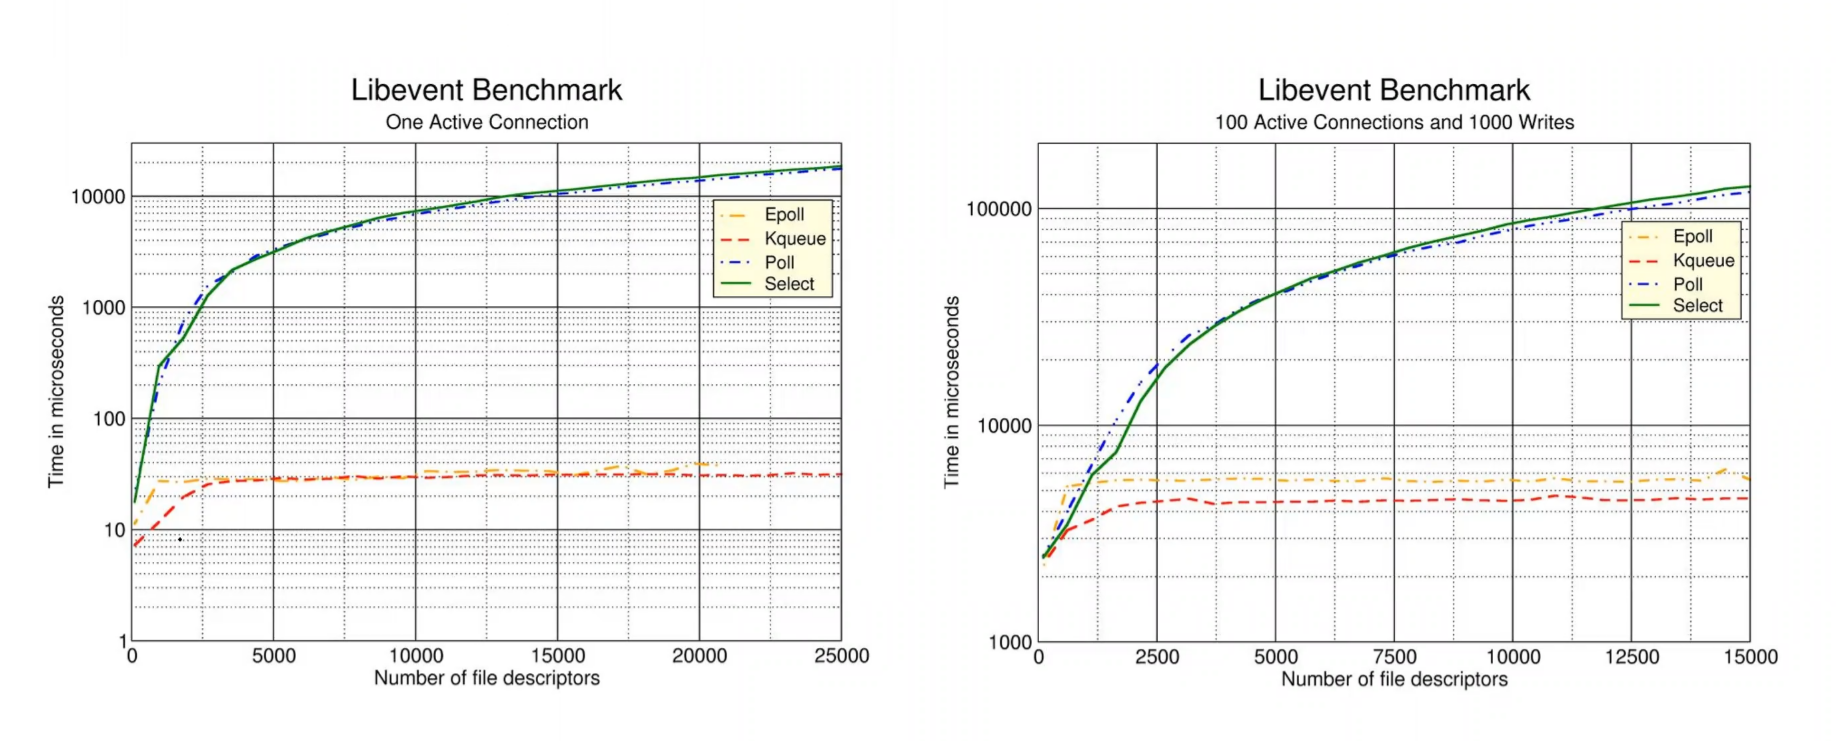
\includegraphics[width=\textwidth]{img/1-epoll-vs-select.png}
		\caption{Performance of \texttt{epoll} vs. \fkt{select}}
		\label{img-1-epoll-vs-select}
	\end{figure}

	\subsection{TCP Options and Packetization}
	\label{tcp-options-and-packetization}
	
	TCP needs to decide important questions: 
	\begin{enumerate}
		\item When to wait for more data from user space
		\item When to send queued data
	\end{enumerate}
	
	If not done so, every \fkt{send} results in a packet. If only one byte is send, that would result in packages with 40 bytes of overhead, but only one byte of payload.

	\subsubsection{Nagle's Algorithm}
	\label{nagles-algorithm}
	
	\begin{algo}{Nagle's Algorithm}
		This algorithm is default TCP socket behaviour.

		Small chunks are accumulated and send, when previous data was ACKed.
		\begin{lstlisting}[language=C]
			if (there is new data to send) {
				if (window size >= max(segment size) && available data >= max(segment size)) {
					complete max(segment size) and send now;
					queue remaining data;
				}
				else if (exists(data in flight waiting to be ACKed)) {
					queue data and send when ACK is received;
				}
				else {
					send data immediately;
				}
			}
		\end{lstlisting}
		\tcblower
		\textbf{Note:} This algorithm is not suited for every application, as it may wait, when an immediate send might be necessary.
	\end{algo}
	
	Disable with \texttt{TCP\_NODELAY} with \fkt{setsockopt}.

	\subsubsection{Delayed ACKs}
	\label{delayed-acks}

	Basic idea: when data is received, we will want to send data as a response.
	Piggy back ACKs for previous data on data you want to send.
	The maximum delay is \( \leq 0.5 \textit{s} \).
	At least every second packet with MSS is ACKed immediately.
	
	This also is TCP default behaviour.
	However, don't combine with \cref{nagles-algorithm}, this may lead to unnecessary waiting times of up to 0.5 \textit{s}. 
	
	Disable with \texttt{TCP\_QUICKACK} with \fkt{setsockopt}.

	Also possible: packetize TCP yourself, using \texttt{TCP\_CORK}, which works best with \texttt{TCP\_NODELAY}.
	It will still send out MSS packets immediately.
	Allows for application level flushing.

	Can also be achieved with \fkt{send} and its \texttt{flags}, by adding \texttt{MSG\_MORE} to it.

	\subsubsection{TCP Fast Open}
	\label{tcp-fast-open}
	
	Normal TCP has 1 RTT delay due to 3-way handshake.

	This option adds the TCP request to TCP's \texttt{SYN} message.
	Leads to 5-7\% speed-up. 

	\textbf{Problems:}\\
	Don't process request before handshake is compelete: risk to security, if handshake would not be completed. Possible DoS scenarios:
	\begin{itemize}
		\item Resource exhaustion attack – Leave connection half open with \texttt{SYN}-flood	
		\item Reflection attack – Spoof live IP addresses, so those get spamed
	\end{itemize}
	Also problem with duplicated data. This also makes the above attacks easier.

	\textbf{Avoiding those problems:}\\
	What to do to tackle the problems
	\begin{itemize}
		\item Keep verified hosts on a \textit{secure} whitelist
		\item Only trust peers that completed a handshake – this needs a proof
		\item Application must tolerated duplicated \texttt{SYN} data
	\end{itemize}

	\begin{figure}[H]
		\centering
		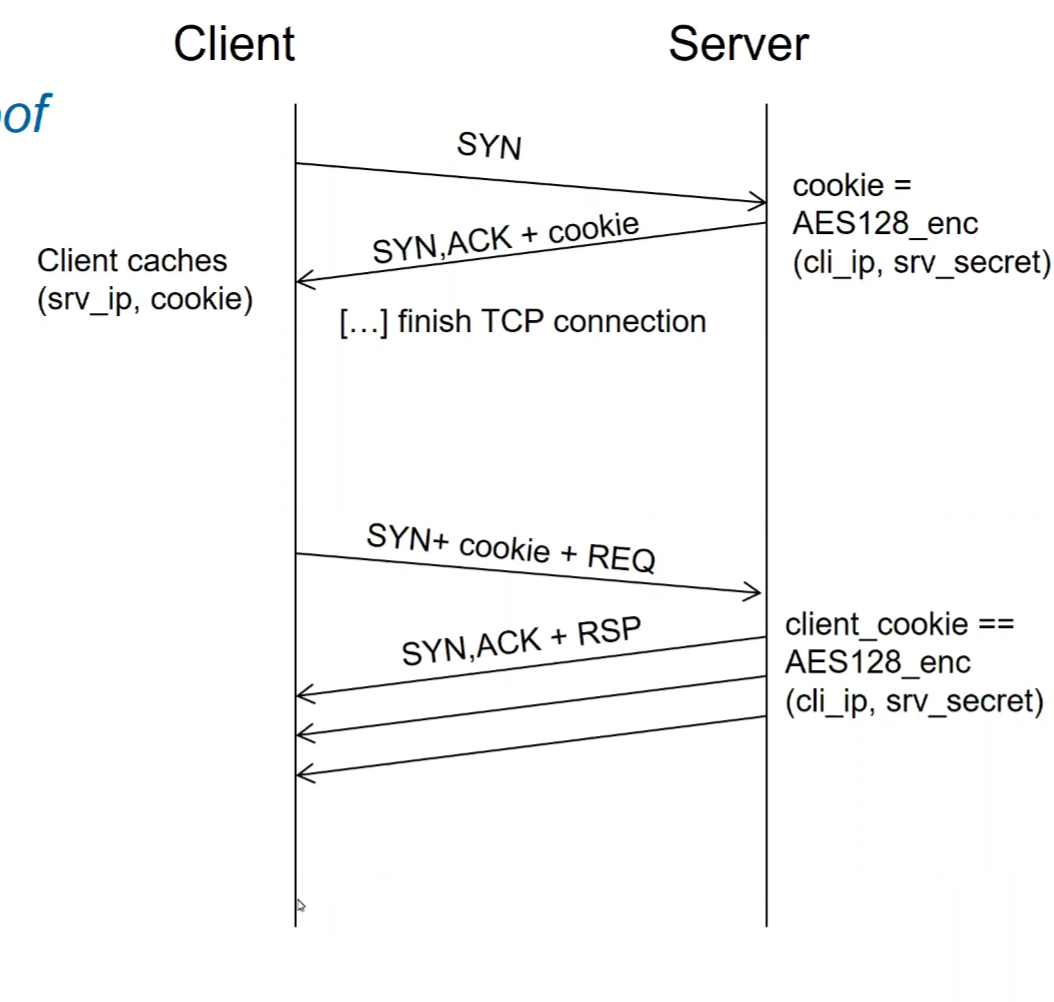
\includegraphics[width=0.65\textwidth]{img/1-tcp-fastopen-proof.png}
		\caption{Using cookie as proof of validity of connection}
		\label{img-1-tcp-fastopen-proof}
	\end{figure}

	Cookies are not valid forever. If cookie is invalid continue with normal TCP handshake.
	
	Cookies may not reach destination. 
	Can be dropped by middleboxes, also timeouts can occur.
	Cookies can be stolen \( \rightarrow \) Rediraction attacks 
	Cookies are dependent on the IP address of the client \( \rightarrow \) change in networks invalidates the cookie, so mobile usage is not optimal

	TCP fast open is not used today, as it leads to more problems than it solves.
	It also has significant problems with middleboxes.

	Activating TCP fast open on servers using \fkt{setsockopts} with \texttt{TCP\_FASTOPEN} together with a maximum count of connections.

	Activating TCP fast open for clients by piggybacking data to the connect call. 
	Also need to use \texttt{MSG\_FASTOPEN}.

	\subsubsection{Multipass TCP}
	\label{multipass-tcp}

	Enable multiple connections between clients and servers. 
	This enables for some backup paths, if one connection suddenly fails.
	However, TCP is \textit{single-path} only, meaning there can only be one connection per socket.
	This leads to poor performance for mobile users, if, for example, if you change from WiFi to 4G networks.

	How to use multi-path TCP:
	\begin{enumerate}
		\item Send options \texttt{MP\_CAPABLE} with \texttt{SYN} message to signal multi-path capability.
		\item If servers sends the same option back, both parties know, that the other party supports 
		\item Send specific \texttt{JOIN} with another \texttt{SYN} message to server, signalling to which connection to join the incoming one to.
	\end{enumerate}

	Again, there are problems with middle boxes.
	Middleboxes (esp. NAT) may \textbf{change} the following field in the IP header.
	\begin{itemize}
		\item IP source address
		\item IP destination address
		\item Source port
		\item Destination port
		\item Sequence number 
		\item ACK number
	\end{itemize}
	They especially can remove the \texttt{MP\_CAPABLE} flag, which leads to unsuccessful connection establishment \( \rightarrow \) normal TCP connection established.

	Also, non-sequential ACKs (when only looking at one path) may be dropped.
	
	Middleboxes may also change all other possible fields, but those changes are not common.
		
	\newpage
	\section{Design Patterns}
	\label{design-patterns}
	
	This chapter describes, how to design networking protocols properly, such that they can be extended and worked with nicely. 

	General design principles are
	\begin{description}
		\item[Simplicity] – Modular structure, with each module implementing a specific task
		\item[Modularity] – Tool for the above
		\item[Well-formedness] – Respecting system boundaries as memory capacity, defined state after errors, adapt to changes within limits
		\item[Robustness] – Protocol can always be exectuted
		\item[Consistency] – avoiding deadlocks, endless loops without progress
	\end{description}

	These lead to the 10 rules of design.

	\begin{defi}{10 rules of design}
		There are 10 rules, that every desing process regarding protocols must follow.
		\tcblower
		\begin{enumerate}
			\item Define the problem well
			\item Define the service first
			\item Design external functionality first, then internal
			\item Keep it simple
			\item Do not connect what's independent
			\item Don't impose irrelevant restrictions
			\item Build high level prototyp and validate first
			\item Implement, evaluate and \textbf{optimize} the design
			\item Check equivalence of prototyp and implementation
			\item Don't skip 1-7
		\end{enumerate}
	\end{defi}

	\subsection{Layering}
	\label{ss-layering}

	Layering describes a modular structure of a protocol, each layer being responsible for a distinct task.

	\begin{halfboxl}
		\textbf{Advantages}
		\begin{itemize}
			\item Smaller subproblems to handle on each layer
			\item Implementation as modules
			\item Exchangeable modules
			\item Reusable modules
		\end{itemize}
	\end{halfboxl}%	
 	\begin{halfboxr}
		\vspace{-\baselineskip}
 		\textbf{Disadvantages}
		\begin{itemize}
			\item Information is hidden \( \rightarrow \) performance loss
			\item Redundantly implemented functionality on different layers
		\end{itemize}
 	\end{halfboxr}

	\textit{Cross-layer communication} can help with redundancy, but is not common, as it is hard to change. 

	\subsection{Protocol Elements}
	\label{ss-protocol-elements}
	
	\subsubsection{Addressing Communication Parties}
	\label{sss-addressing-communication-parties}
	
	All communicating parties need to be identifiable within the network. 
	Therefore, a unique identifier is needed for every party.
	You have to keep in mind address size, to be safe in the future.
	It may be possible to introduce an option to extend the address space.
	
	Typically, single parties are identified, but it may also be useful to group mutiple data flows into one connection.

	\paragraph{RTP Flow IDs}
	\label{pgf-rtp-flow-ids}
	
	The RTP (\textit{Real-time Transport Protocol}) is capable of grouping flows.

	\begin{figure}[H]
		\centering
		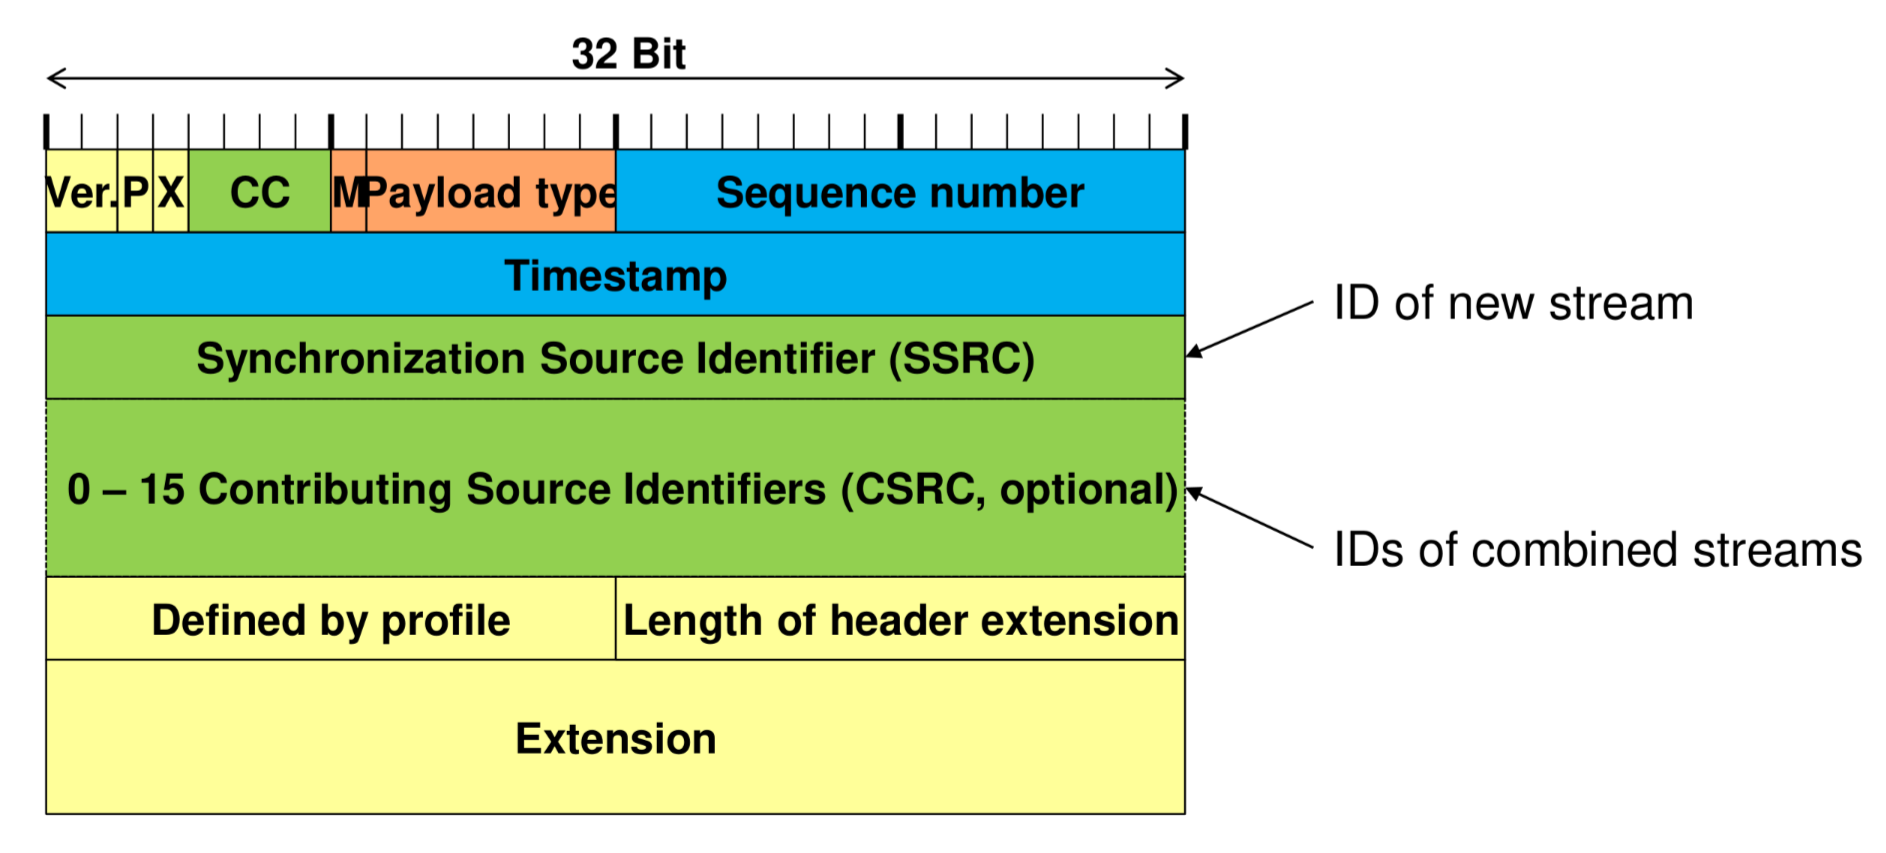
\includegraphics[width=\textwidth]{img/2-rtp-flow-ids.png}
		\caption{RTP header for grouping flows}
		\label{img-2-rtp-flow-ids}
	\end{figure}

	\subsubsection{Sequence Control}
	\label{sssec-sequence-control}
	
	This is necessary in order to be able to asure, that packets are received in the correct order or in which order to process incoming packets.
	This commonly uses \textit{sequence number}.
	Again, consider the maximum length of sequence number fields in your protocol header.
	What to do when you run out of sequence numbers to use?

	\subsubsection{Flow Control}
	\label{sssec-flow-control}
	
	Adapt transmit speed to clients abilities.
	Popular approaches are 
	\begin{itemize}
		\item Stop-and-wait – end2end
		\item Sliding window – hop2hop
	\end{itemize}

	General advice: Orient around RTT and only consider bandwidth reservation if resources are scalable w.r.t. number of communication parties.

	Example: Transmission Rate Control (\textit{TRC}).
	It uses the idea of applying flow control on multiple protocol layers simultaneously.

	\subsubsection{Access and Congestion Control}
	\label{sssec-access-and-congestion-control}
	
	One need to consider how to avoid network overload, and what to do, if overloading is not avoidable.

	In local networks, \textit{medium access control} is used, in global networks \textit{congestion control}.

	Might be necessary to violate layering approach, as is done for TCPs \textit{Explicit Congestion Control}.

	Congestion control can be done on application layer by scaling down resolution of content (bitrate, lower resolution of video, etc.).
	May change based on messages from the client. 
	Alternatively use \textit{interarrival time} between packets and packet loss ratio (UDP only).

	\subsubsection{Error Control}
	\label{sss-error-control}
	
	There often is the need to detect and correct corrupted packets in order to minimize packet loss.

	General types of error correction methods are:
	\begin{description}
		\item[Automatic Repeat Request \textit{ARQ}] On error, rerequest the packet. ACK or ACK/NACK approaches
		\item[Forward Error Correction \textit{FEC}] Add redundancy to packets, use sophisticated methods such as CRC to correct them
	\end{description}

	TCP uses ARQ, but emulates a NACK with two consecutive ACKs for the same packet.

	\textit{Selective ACKs} can be used to acknowledge ranges of sequence numbers \( \rightarrow \) more efficient acknowledging

	\paragraph{Retransmission Schemas for ARQ}
	\label{pgf-retransmission-schemas-for-arq}
		
	There are three main methods used for retransmission.

	\begin{figure}[H]
		\centering
		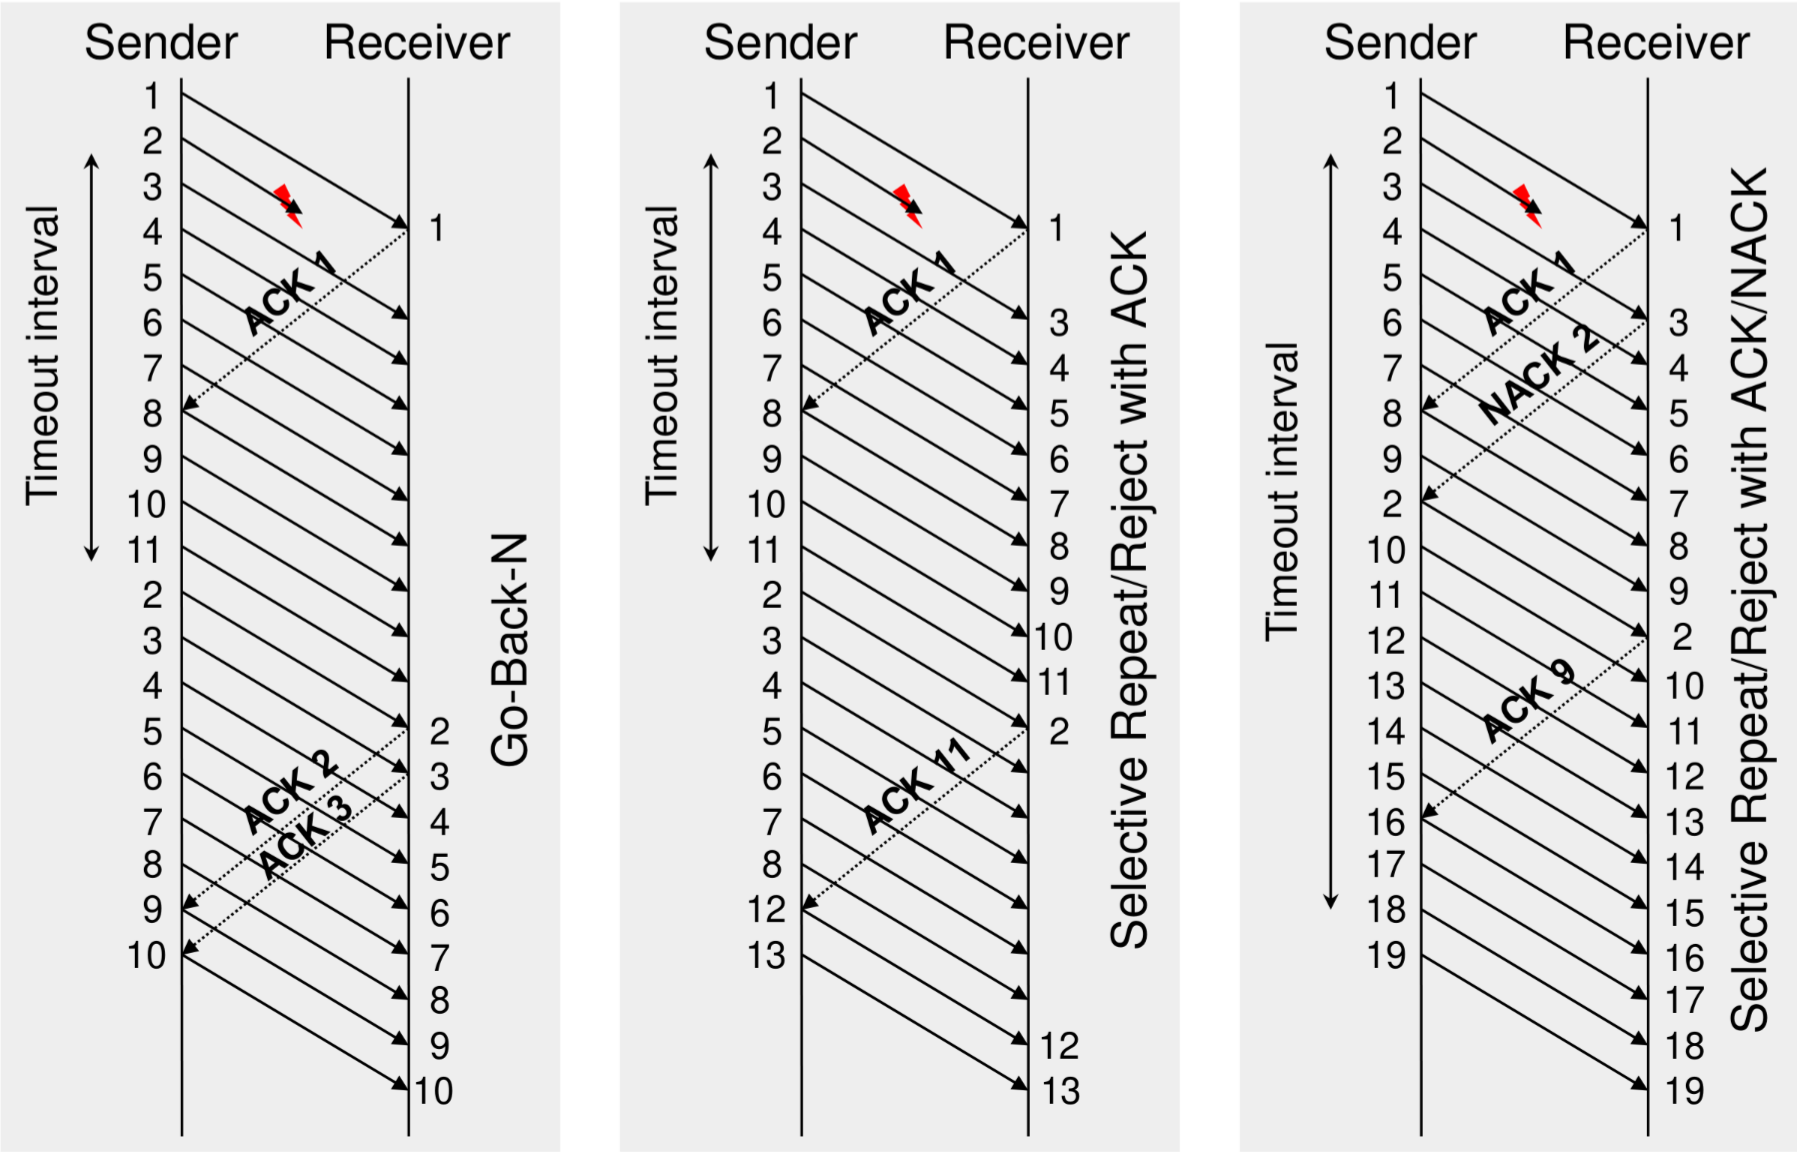
\includegraphics[width=\textwidth]{img/2-retransmission-schemas.png}
		\caption{All introduced retransmission schemas}
		\label{img-2-retransmission-schemas}
	\end{figure}

	\begin{thirdboxl}
		\vspace{-\baselineskip}
		\begin{defi}{Go-back-N}
			Retransmit all non-ACKed packages after a timeout occurs.
		\end{defi}
	\end{thirdboxl}
	\begin{thirdboxm}
		\vspace{-\baselineskip}
		\begin{defi}{Selective Repeat/Reject with ACK}
			Commulative acknowledgement for all packages up to, in this case 11. 2 gets resend, as a timeout for the ACK for 2 occurs on the server side. All packets 3 through 11 are buffered, but partially retransmitted by the server nontheless.
		\end{defi}
	\end{thirdboxm}
	\begin{thirdboxr}
		\vspace{-\baselineskip}
		\begin{defi}{Selective Repeat/Reject with ACK and NACK}
			Basically the same as selective repeat/reject with ACK, but NACK all missing packets upon receiving the next packet.
		\end{defi}
	\end{thirdboxr}

	Use stop-and-wait only in cases with low RTT or where error rates are really low.

	Use go-back-n if the receiver is very limitted.

	Use any selective method in any other case.

	\textit{NACK-only} strategies do not work in \enquote{normal} operation, they however work in high-throughput, high-reliability networks. 
	This is due to the problem, that NACKs are not able to signal the reception of messages, only obviously missing packets.
	This way, missing of the last packet of a stream cannot be detected, as the client does not know that another packet was send, which does not generate a NACK which would signal to the server, that the last packet has gone missing.

	\paragraph{Forward Error Correction Schemas}
	\label{pgf-forward-error-correction-schemas}
	
	Send all packets \( n \) times, to be able to correct corrupted packets. 

	Redundancy per packet, i.e. with Hamming-Codes can also be used.

	Also guessing what the lost packet contents were can be done, it smaller errors in some packets is not too bad. May be done by interpolating past packets.

	\begin{defi}{XOR-redundancy}
		Combine \( n \) packets into one XORed packet and send it as well.
		XOR-redundancy is capable of restoring one packet.
		However the clients ability to process packets in a fastly manner must be considered, as only \textbf{exactly} one packet can be reconstructed.
	\end{defi}

	\begin{figure}[H]
		\centering
		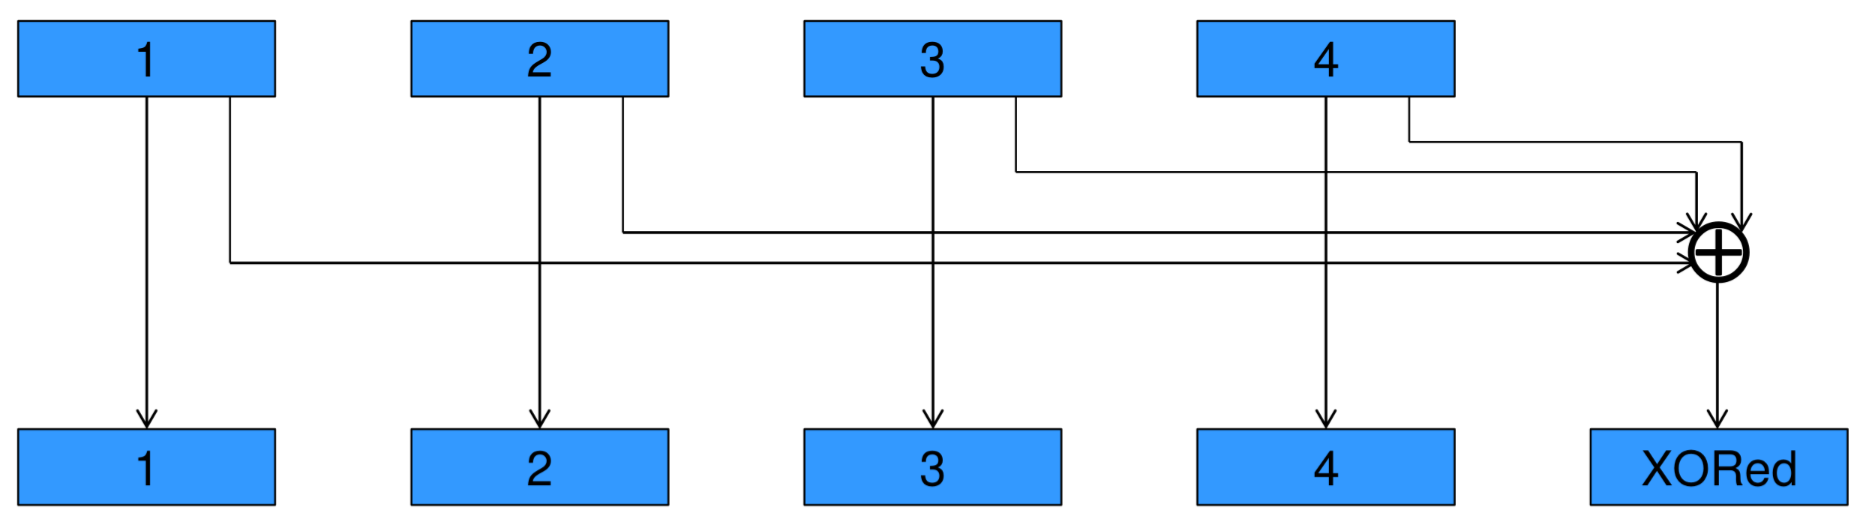
\includegraphics[width=\textwidth]{img/2-xor-redundancy.png}
		\caption{XOR-redundancy}
		\label{img-2-xor-redundancy}
	\end{figure}	

	Interleaving redundancy packets and original packets can lead to the ability of restoring \( n \) sequenced packets.
	
	\begin{defi}{Hamming correction}
		Insert parity bits at positions that are labeled with a power of 2.
		Start counting with 1.
		This blows up the original message by \( \log_2(|\texttt{message}|) \).
		A parity bit \( n \) is calculated by adding all positions, that in their binary representation, have a 1 in position \( \log_2(n) \).
		\tcblower
		Let \( D \) be the hamming distance of two strings.
		Then a \( t \) errors can be corrected, if \( D \geq 2t + 1 \), and \( t \) errors can be detected, if \( D \geq t + 1 \).
	\end{defi}

	Limitation: Hamming distance of 3 required, to be able to correct one error.

	\begin{alertbox}
		Be aware, that \textbf{BCH} codes do not seem to be relevant for the exam and are therefore not included in detail here.
		\tcblower
		You don't have to be able to calculate BCH codes!
	\end{alertbox}

	\begin{defi}{Bose, Chaudhuri, Hocquenghem Code (\textit{BCH})}
		Let 
		\begin{itemize}
			\item \textit{block length} be \( n = 2^m -1 \)
			\item \textit{number of parity bits } be \( p = n - k \leq m \cdot t \)
			\item \textit{minimum distance} be \( d_{min} \geq 2t + 1 \),
		\end{itemize}
		with \( t < 2^{m} - 1 \) and \( m \geq 3 \). 
		Then \( t \) is the number of errors that can be corrected. 
		\tcblower
		This is not a complete defintion. 
		BCH codes are a family of codes, where each instance can be specified by giving a tuple.
	\end{defi}
	BCH functions more or less like CRC.
	
	\begin{defi}{Reed-Solomon Code}
		Able to deal with burst errors, basically a non-binary BCH code. It generates less overhead then BCH codes. Let
		\begin{itemize}
			\item \textit{block length} be \( n = q-1 \)
			\item \textit{number of parity bits} be \( n - k= 2 \cdot t \)
			\item \textit{minimum distance} be \( d_{min} = 2t + 1 \),
		\end{itemize}
		where \( q \) is any power of any prime \( p \), then \( t \) errors can be corrected.
	\end{defi}

	Ignoring checksums might be a valid way to minimize paket loss, if application can tolerate errors.

	\textit{Refector} makes use of this approach, with an opt-in mechanism.
	It is used on the end hosts.
	Analogy: Postmen can handle wrongfully addressed letters to a certain degree.
	Refector does the same, and can therefore handle minimally corrupted headers.
	The \enquote{correct} application is found by choosing the one with the minimal hamming distance to the received header. 
	There are some field in the IP header, that can be ignored in the process, such as \textit{Version}.
	The protocol build on UDP.
	It reduces packet loss up to 25\%.

	\subsubsection{Encodings}
	\label{sss-encodings}
	
	The focus here lies mainly on compression.

	There are two variants: Lossy and loss-less compression.

	Lossy compression is highly recommended for video streams, as small pixel errors are not recognizable by the human eye.
	
	\paragraph{Lossless Compression}
	\label{pgf-lossless-compression}

	Again, two main methods:
	\begin{enumerate}
		\item remove redundancy: compress sequences of the same symbol 
		\item statistical analysis: statistically construct the optimal compression scheme
	\end{enumerate}
	
	\begin{defi}{Run-length encoding \textit{RLE}}
		Basically compress all sequences \texttt{AAAAAAAAA} \( \rightarrow \) \texttt{A!9} and so on.
	\end{defi}

	\begin{defi}{Differential Enconding}
		Instead of storing the values themselves, encode the distance to the nearest other datapoints.
	\end{defi}

	\begin{algo}{Lempel-Ziv-Welch Encoding (LZW)}
		Building a dictionary for phrases during encoding of the data.
		\tcblower
		\( D = \set{\texttt{All unique symbols in the data stream}} \)

		\( E = \set{d_i \rightarrow e_i \mid d_i \in D, e_i \in \nat \texttt{ unique}} \)
		
			Start at the \( 1^{\text{st}} \) position (\( i = 1 \))	of the plain text \( w = w_1w_2\cdots w_n \).
		\begin{enumerate}
			\item Encode \( w_{i}, \dots, w_{i+k-1} \) with longest match in \( E \) as \( e_j \) with \( |e_j| = k \).
			\item Add \( e_jw_{i+k} \) to \( D \) and a corresponding encoding to \( E \).
			\item Move to position \( i + k \).
			\item Repeat until done.
		\end{enumerate}	
	\end{algo}
	
	We now will continue with \textbf{statistical analysis}.

	\begin{defi}{Entropy}
		\textbf{Information per symbol}
		\( I_i = -\log_{2}(p_i) \)

		\textbf{Entropy for whole word}
		\( H = \sum_{i=1}^n p_i \cdot I_i \)

		with \( p_i \) is the probability of \( i \) appearing.
		\tcblower
		\enquote{How much information is carried by each symbol?}
	\end{defi}

	This is used for \textit{Huffman Code}.

	\begin{algo}{Huffman Code}
		Encode a data stream in a binary tree, starting with the leafes.

		\textbf{Input:} Data stream.

		\textbf{Returns:} Optimal encoding w.r.t. entropy.
		\tcblower
		\begin{enumerate}
			\item Assign each symbol of your alphabet the probability, with which it occurs in the data stream. Add mapping to a set.
			\item Add two mappings \( a \rightarrow p(a) \) and \( b \rightarrow p(b) \) with lowest probability from your set to the tree. Remove them from the set. Left: smaller prob.
			\item Add a parent node \( ab \rightarrow p(a)+p(b) \).
			\item Add generated mapping to set.
			\item Repeat until set is empty.
		\end{enumerate}
		\alert{Always choose \textit{prefix free} code words.}
	\end{algo}

	The resulting code, which is generated by traversing the tree, can be evaluated w.r.t. entropy: 
	\begin{enumerate}
		\item Compute information per symbol
		\item Calculate entropy of the system, \( H_\texttt{theory} \)
		\item Calculate entropy of the code like \(H_\texttt{code} = \sum_{i=1}^n p_i \cdot |\texttt{code}_i| \) 
		\item Compare the two entropies
	\end{enumerate}
	
	However, Huffman code cannot guarantee the smallest code size (\( H_\texttt{code} \approx H_ \texttt{theory} \)).

	\begin{algo}{Arithmetic Encoding}
		Encode data as a value between \( [0,1]_\reals \)
		\tcblower
		Assign each symbol a corresponding probability again.
		Start at position \( i = 1 \) of the data stream \( w =w_{1}w_{2}\dots w_{n} \).
		\begin{enumerate}
			\item Divide the assigned interval (see figure below), that matches \( p_{w_{1}\dots w_i} \) into smaller segments, corresponding to \( p_{w_{1}\dots w_i} \cdot p_{s}\), where \( p_s \) is the probability of symbol \( s \) occuring.
			\item Choose the subsegment (which is \( w_{1}\dots w_i \cdot s \)), that matches \( w_{1}\dots w_{i+1} \) of your data stream
			\item Increase \( i \) and continue until all is done.
		\end{enumerate}
		Then, with \( p_{w_{1}w_{2}\dots w_n} = p \), the data can be encoded using only \( \ceil*{-\log_{2}(p)} \) bits.
	\end{algo}

	\begin{figure}[H]
		\centering
		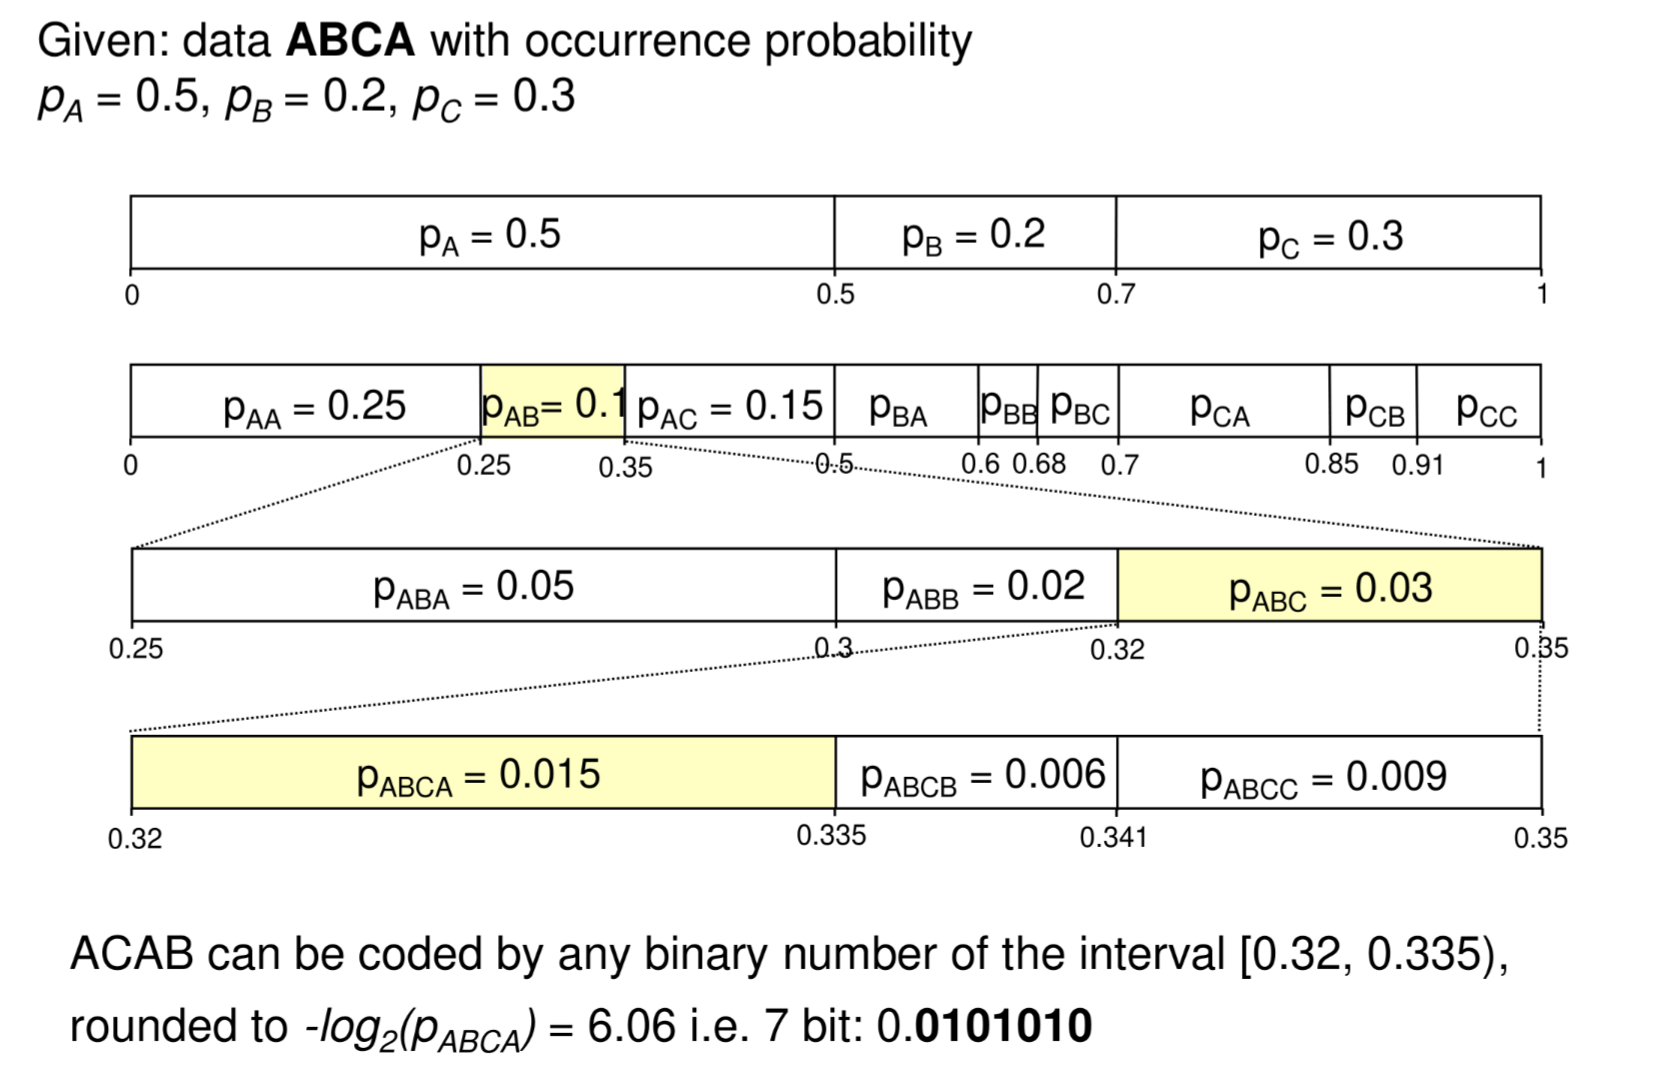
\includegraphics[width=\textwidth]{img/2-arithmetic-encoding.png}
		\caption{Example of arithmetic encoding}
		\label{img-2-arithmetic-encoding}
	\end{figure}

	\subsection{Protocol Design Aspects}
	\label{ss-protocol-design-aspects}

	\subsubsection{Connection Type}
	\label{sss-connection-type}
	
		You have to decide, if you want to design a \textit{connectionsless} or \textit{connection-oriented} protocol. 
	Rule of thumb: The more controll parameters are nedded, the higher the chance you need connection oriented protocols.
	
	If single commands will all fit in one UDP packet, would be alright as well.

	UDP is also better suited for real-time and/or interactive applications, as it is much faster.
	
	\subsubsection{Signaling}
	\label{sss-signaling}
	
	Before, during and after connections, signalling must be done.
	This includes \textit{status information}, \textit{parameters of the connection}, specific to this connection and so on.

	\begin{defi}{Out-of-band signalling}
		There are separate control and data streams.
		They may be implemented in two seperate protocoll \enquote{phases}, or on different ports.
		One could even use different protocols for control and data streams.

		Is able to provide QoS.
		\tcblower
		For example \textit{SIP}.
	\end{defi}

	\begin{defi}{In-band signalling}
		There is \textbf{no} separate control stream, but a combined data and signal stream.
		\tcblower
		For example \textit{TCP}.
	\end{defi}

	\subsubsection{Maintaining Network State}
	\label{sss-maintaining-network-state}
	
	Protocols may store states in the network on nodes in the path between to parties.

	\paragraph{Hard State Maintaining}
	\label{pgf-hard-state-maintaining}
	
	State changes only with dedicated control messages.

	Requires really reliable signalling.
	Checks, if a node is still alive has to be performed from time to time.

	Example: TCP \( \rightarrow \) \texttt{FIN} messages needed to terminate connections.

	\paragraph{Soft State Maintaining}
	\label{pgf-soft-state-maintaining}
	
	Timeouts may delete a state. 
	Must be refreshed to be kept alive.

	\alert{This is almost always the approriate maintaining method!}

	Both state maintaining methods may implement the other one for certain things, s.t. some protocols use a mixture.

	\subsubsection{Control of Communication}
	\label{sss-control-of-communication}
	
	\begin{halfboxl}
		\textbf{Centralized Control}
		\begin{itemize}
			\item Easy to program and debug
			\item Ex.: Client/Server 
		\end{itemize}
	\end{halfboxl}%
	\begin{halfboxr}
		\vspace{-\baselineskip}
		\textbf{Decentralized Control}
		\begin{itemize}
			\item More robust, no single point of failure
			\item Harder to implement
			\item Ex.: P2P
		\end{itemize}
	\end{halfboxr}
	
	A mixed approach is \textit{Software Defined Networking (SDN)}.

	\begin{figure}[H]
		\centering
		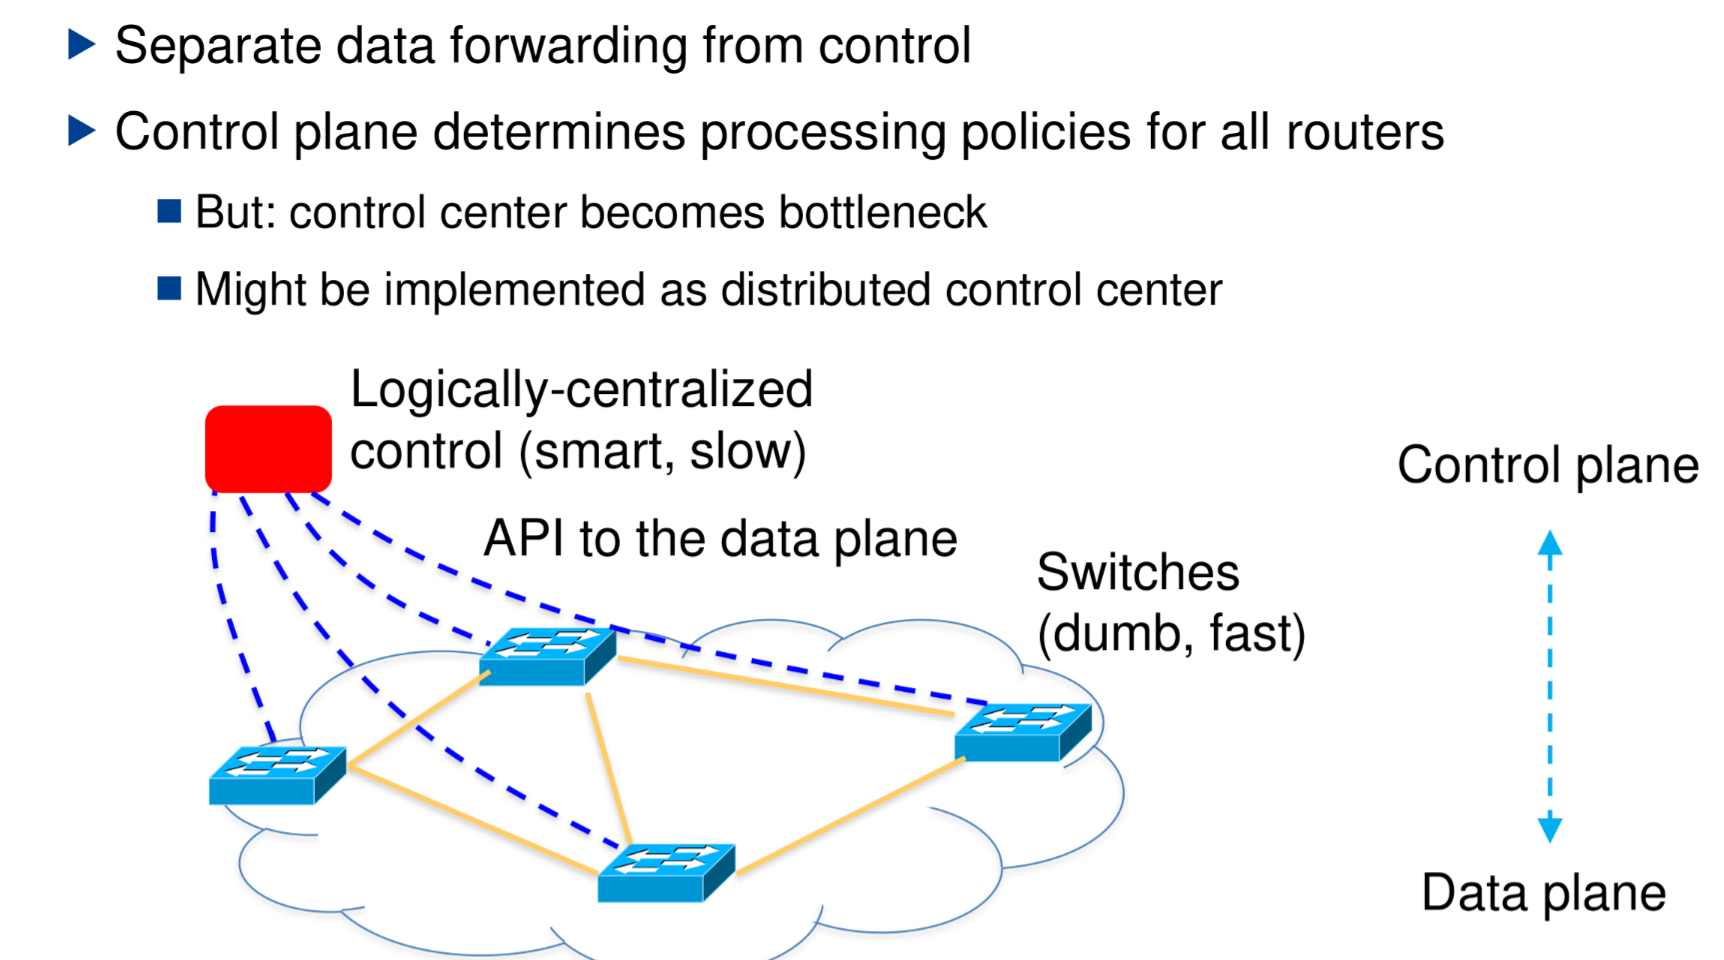
\includegraphics[width=\textwidth]{img/2-sdn.png}
		\caption{Software defined networking}
		\label{img-2-sdn}
	\end{figure}


	\subsubsection{Randomization of Protocols}
	\label{sss-randomization-of-protocols}
	
	Useful to make sequence numbers non-predictable, making it more secure.

	CSMA/CD uses random waiting times on errors, to avoid consecutive collisions.

	\begin{defi}{Random Early Discard}
		Throw away packets, \textbf{before} buffer capacity is reached.
		\begin{figure}[H]
			\centering
			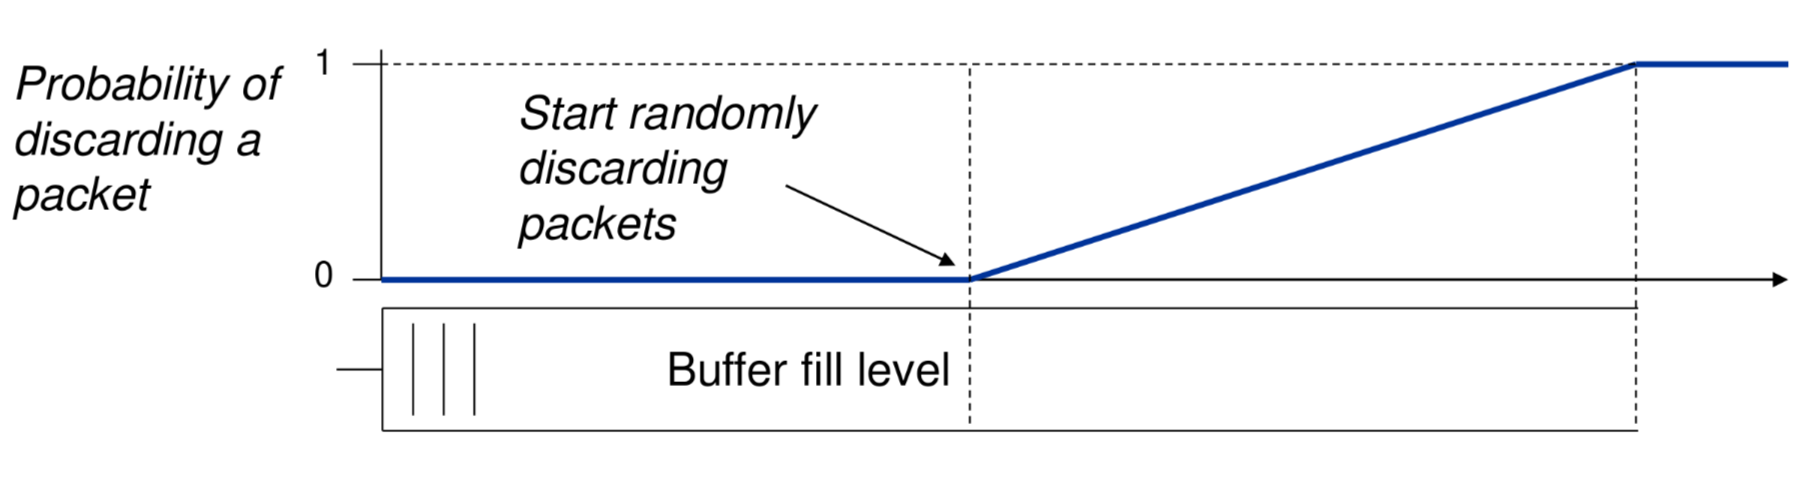
\includegraphics[width=\textwidth]{img/2-red.png}
			\caption{Random Early Discard}
			\label{img-2-red}
		\end{figure}
	\end{defi}
	
	\textit{Zmap} also makes use of this, in order to scan a complete network without being blocked by service providers, as scanning the addressspace linearly would result in a block.

	\subsubsection{Indirection}
	\label{sss-indirection}
	
	\begin{center}
		\enquote{Every problem in Computer Science can be solved by another layer of indirection.}
	\end{center}

	\paragraph{Multicast}
	\label{pgf-multicast}
	
	Multicast makes use of \textit{indirection}:
	\begin{itemize}
		\item Client sends packet to address of multicast group
		\item Routers and middleboxes in general forward the packet to all clients, that registered for this group
	\end{itemize}

	\paragraph{Content Distribution Network}
	\label{pgf-content-distribution-network}	

	Replicate content on a tree-like structure of other servers. Media servers are mirrors of a main server. 

	Indirection comes from the fact, that all clients use the same address to connect, but are \textit{redirected} to the same server.

	See \texttt{google.com}, there is no single Google server, there are thousands, that distribute the load among themselves.

	Tool to use to achieve this: DNS.
	
	
	\subsection{Design of HTTP}
	\label{ss-design-of-http}
	
	HTTP was designed for documentation exchange between spacially far apart machines. Originally designed to work on simple \texttt{ASCII} strings, terminated by a carriage return.

	\subsubsection{HTTP/0.9}
	\label{sss-http-0.9}
	
		Operates on TCP port 80, and only supports \textit{HTML}.
		Content is send directly, after a correct request was received.
		The connection is immediately closed after servicing a request.

	Some commonly used commands are
	\begin{description}
		\item[GET] Request for content
		\item[PUT] Store document on server
		\item[HEAD] Only request header information
		\item[POST] Append content to webpage
		\item[DELETE] Remove contents from server
	\end{description}
	
	\subsubsection{HTTP/1.0}
	\label{sss-http-1.0}
	
	Introduces \textit{multi-line requests} and \textit{responses}. Response objects are not limited to HTTP anymore.
	
	Content is send after meta information about the contents of the webpage.
	Otherwise basically the same as \cref{sss-http-0.9}. 

	\begin{halfboxl}
		\begin{figure}[H]
			\centering
			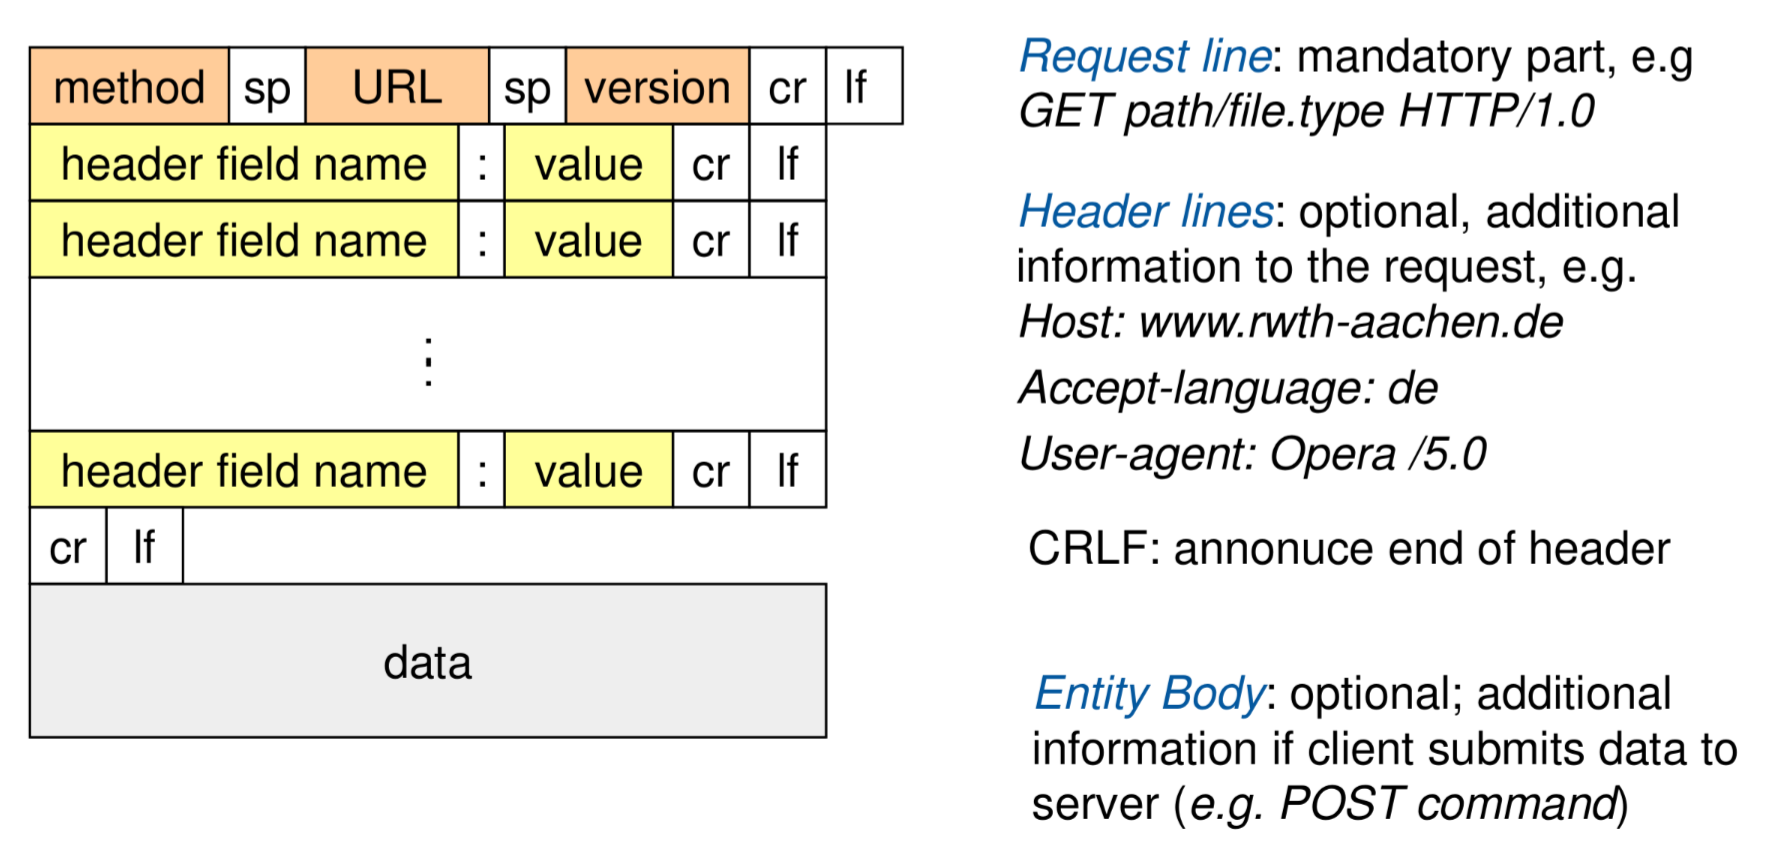
\includegraphics[width=\textwidth]{img/2-http-10-requests.png}
			\caption{Request structure of HTTP 1.0}
			\label{img-2-http-10-requests}
		\end{figure}	
	\end{halfboxl}%
	\begin{halfboxr}
		\begin{figure}[H]
			\centering
			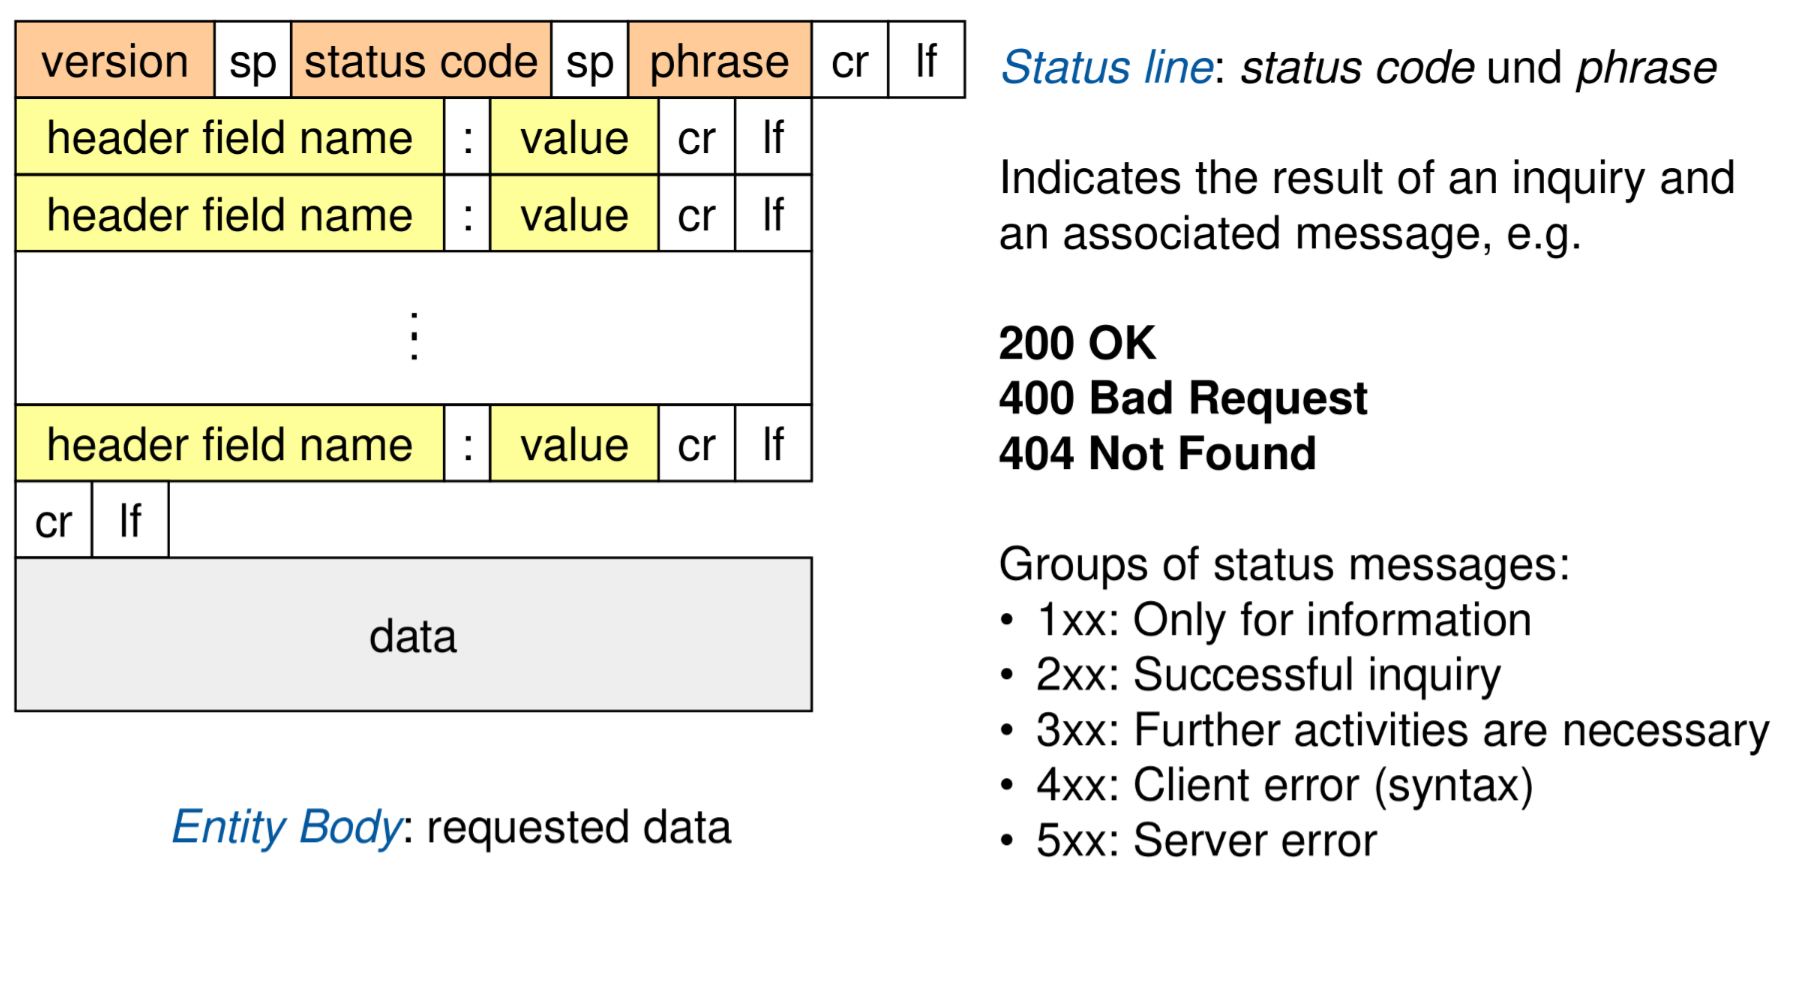
\includegraphics[width=\textwidth]{img/2-http-10-response.png}
			\caption{Response structure of HTTP 1.0}
			\label{img-2-http-10-response}
		\end{figure}
	\end{halfboxr}
	
	\subsubsection{HTTP/1.1}
	\label{sss-http-1.1}
	
	In comparisson to \cref{sss-http-1.0}, the following things are extended:
	\begin{itemize}
		\item Request method
		\item Error codes
		\item Headers
		\item List of accepted file types: All types are allowed
	\end{itemize}

	\textit{Cookies} can be used in order to make HTTP stateful.
	Connections are not immediatly closed upon sending out a response. 
	Furhtermore:
	\begin{itemize}
		\item Content encodings and character sets were introduces
		\item Languages can be negotiated
		\item Caching enabled
		\item Cookies introduced
		\item \dots
	\end{itemize}

	\paragraph{Dynamic Adaptive Streaming over HTTP (DASH)}
	\label{pgf-dynamic-adaptive-streaming-over-http}
	
	Method to make HTTP a \enquote{real} streaming protocol.

	\begin{enumerate}
		\item Cut down video file into several smaller chunks and store them in differnt bitrates
		\item Client firstly loads file that contains names of all chunks that need to be downloaded over the course of streaming
		\item Client requests chunks one-by-one, each with its own HTTP request. Bitrate can be adjusted with every request
	\end{enumerate}

	This is \textbf{not} an \textbf{option} of HTTP, but really a use-case of it.

	\paragraph{Head of Line Blocking}
	\label{pgf-head-of-line-blocking}
	
	Allthough HTTP/1.1 uses up to 6 different connections per connection to a webserver, websites still load pretty slowly. Solution: \textbf{Pipelining}. 

	This means that requests are send out directly after each other, without waiting for responses. 

	\begin{figure}[H]
		\centering
		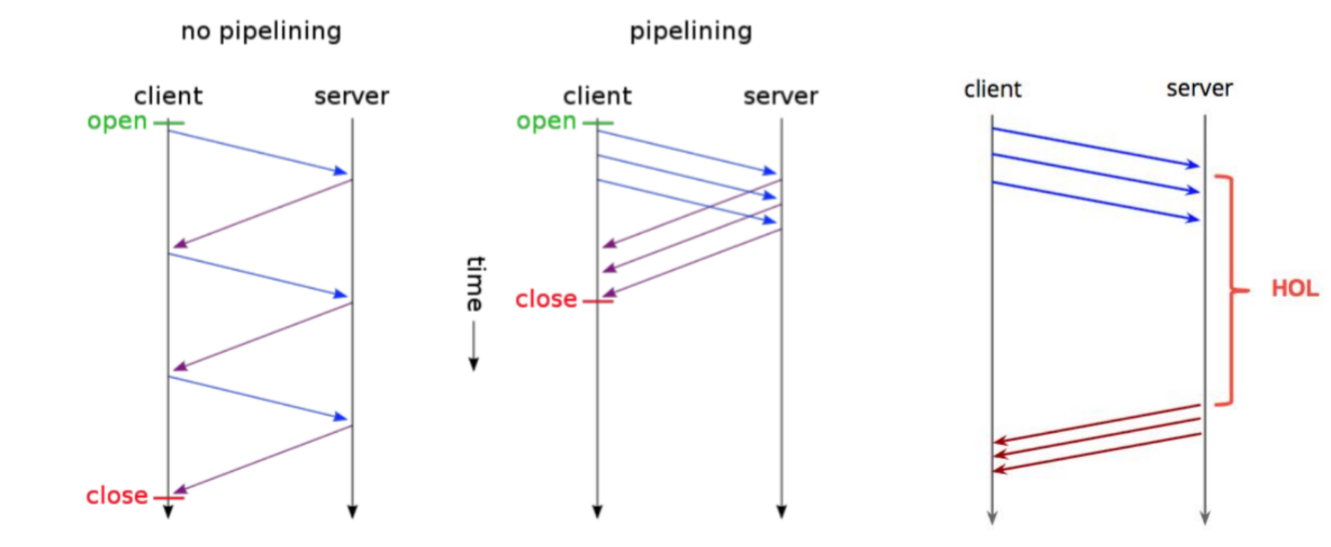
\includegraphics[width=\textwidth]{img/2-hol-pipelining.png}
		\caption{HoL Pipelining}
		\label{img-2-hol-pipelining}
	\end{figure}
	
	However, large requests still slow down loading.

	\paragraph{Domain Sharding}
	\label{pgf-domain-sharding}
	
	Instead of keeping all resources on one webserver, distribute them accross multiple subdomains. 
	\begin{center}
		\texttt{www.example.com} \( \rightarrow \)  \texttt{\( \set{\textit{sub}_{1}, \dots, \texttt{sub}_{n}}\texttt{.example.com} \)}
	\end{center}

	This leads to more DNS lookups, which can also slow down loading, also there are more connections to be kept alive.
	
	If one knows what he is doing, domain sharding can increase throughput. However, most application overuse it, which leads to underused TCP connections and therefore more overhead, which in turn slows down communication again.

	\subsubsection{Spriting Images and Concatenating Files}
	\label{sss-spriting-images-and-concatenating-files}
	
	\begin{halfboxl}
		\textbf{Advantages} 
		\begin{itemize}
			\item Reduces number of overall requests
		\end{itemize}
	\end{halfboxl}%
	\begin{halfboxr}
		\vspace{-\baselineskip}
		\textbf{Disadvantages}
		\begin{itemize}
			\item Waste of bandwidth if not all resources are needed
			\item If one single element is updated, the whole bundle must be acquired again
			\item Sprites require slow parsing
			\item Spritet images need more memory
		\end{itemize}
	\end{halfboxr}

	\( \Rightarrow \) Enjoy with care, there is not much good to it.

	\subsubsection{Resource Inlining}
	\label{sss-resource-inlining}
	
	Idea: Embed resources in webpage itself.

	Inline CSS, JS, even images (using \( \texttt{Base}_{64} \)) and audio can be embedded.

	\begin{halfboxl}
		\textbf{Advantages} 
		\begin{itemize}
			\item Reduces number of overall requests
		\end{itemize}
	\end{halfboxl}%
	\begin{halfboxr}
		\vspace{-\baselineskip}
		\textbf{Disadvantages}
		\begin{itemize}
			\item Waste of bandwidth if not all resources are needed
			\item If one single element is updated, the whole bundle must be acquired again
			\item No reusability of assets, need to be included into every source file that use those resources, which leads to a memory penalty
		\end{itemize}
	\end{halfboxr}

	\subsubsection{HTTP/2}
	\label{sss-http-2}
	
	Goals were not to use as many connections and lower the \textit{perceived} time things take to load, while retaining the high-level semenatics of HTTP/1.1.
	HTTP/2's smallest unit of communication now is a so called \textit{frame}, which are send over \textit{exactly} one connection.
	It also uses binary represenation instead of \texttt{ASCII}.

	\begin{halfboxl}
		\begin{figure}[H]
			\centering
			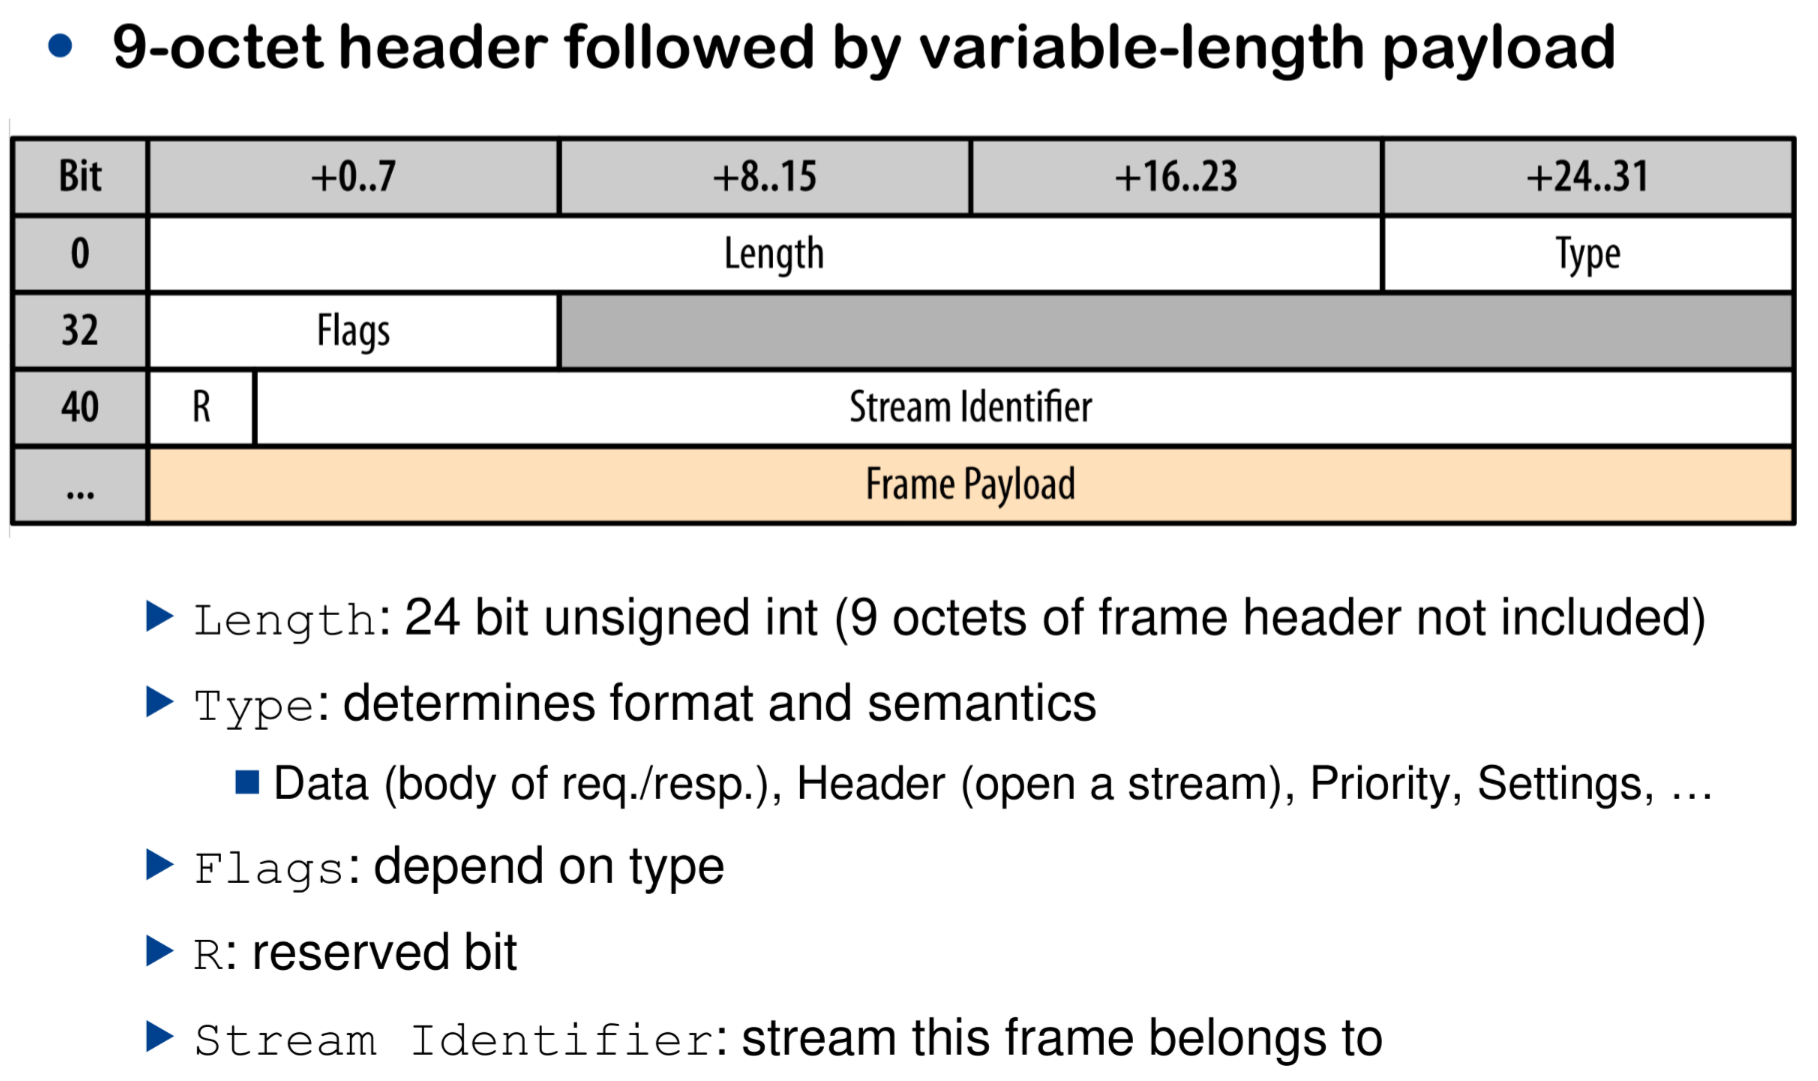
\includegraphics[width=\textwidth]{img/2-http2-frame.png}
			\caption{Frame of HTTP/2 communication}
			\label{img-2-http2-frame}
		\end{figure}
	\end{halfboxl}%
	\begin{halfboxr}
		\begin{figure}[H]
			\centering
			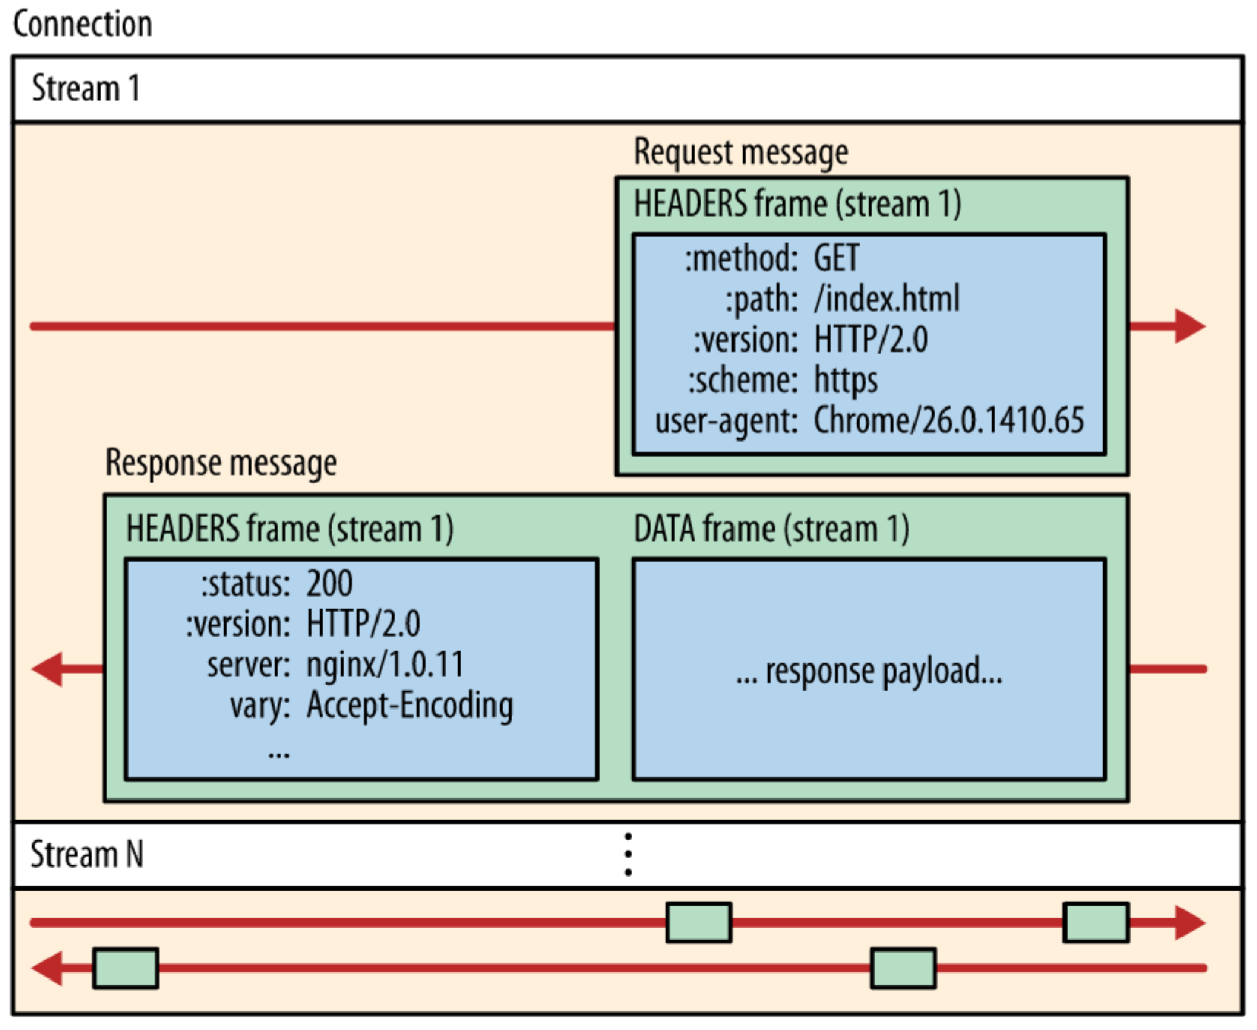
\includegraphics[width=\textwidth]{img/2-http2-conn.png}
			\caption{Layout of connection via HTTP/2}
			\label{img-2-http2-conn}
		\end{figure}
	\end{halfboxr}
	
	HTTP/2 also allows to specify, in which order to download content from the web server. The order is represented by a tree structure. This allows for signal priortization. 

	\alert{This is only a recommendation. The server is not required to follow the requested download order.}

	Also, a server is allowed to \texttt{PUSH} data to the client, without the client requesting it. It can be used to pre-send CSS files and similar data. The server has to announce the push, the client can deny it. Pushed data \textit{has} to come from the same domain, such that no external data can be pushed to the client.

	Is scheduled to be removed from Google services.

	Flow control is supported, but has to be implemented by the application. 
	Additional flow control is useful, as TCP only supports flow control on a per-connection basis. 
	As HTTP/2 supports more than one stream per connection, per-stream flow control can be implemented as well.
	There is no implemenation specified in the standard.

	\paragraph{Header Compression with \texttt{HPACK}}
	\label{pgf-header-compression}
	
	Headers have up to 800 bytes of data, which is repetitive. 
	They are now allowed to be compressed, using Huffman encoding and a combination of static and dynamic tables (see \cref{pgf-lossless-compression}).
	The static table contains codes for the 61 most common headers used in HTTP/2.	
	
	\begin{figure}[H]
		\centering
		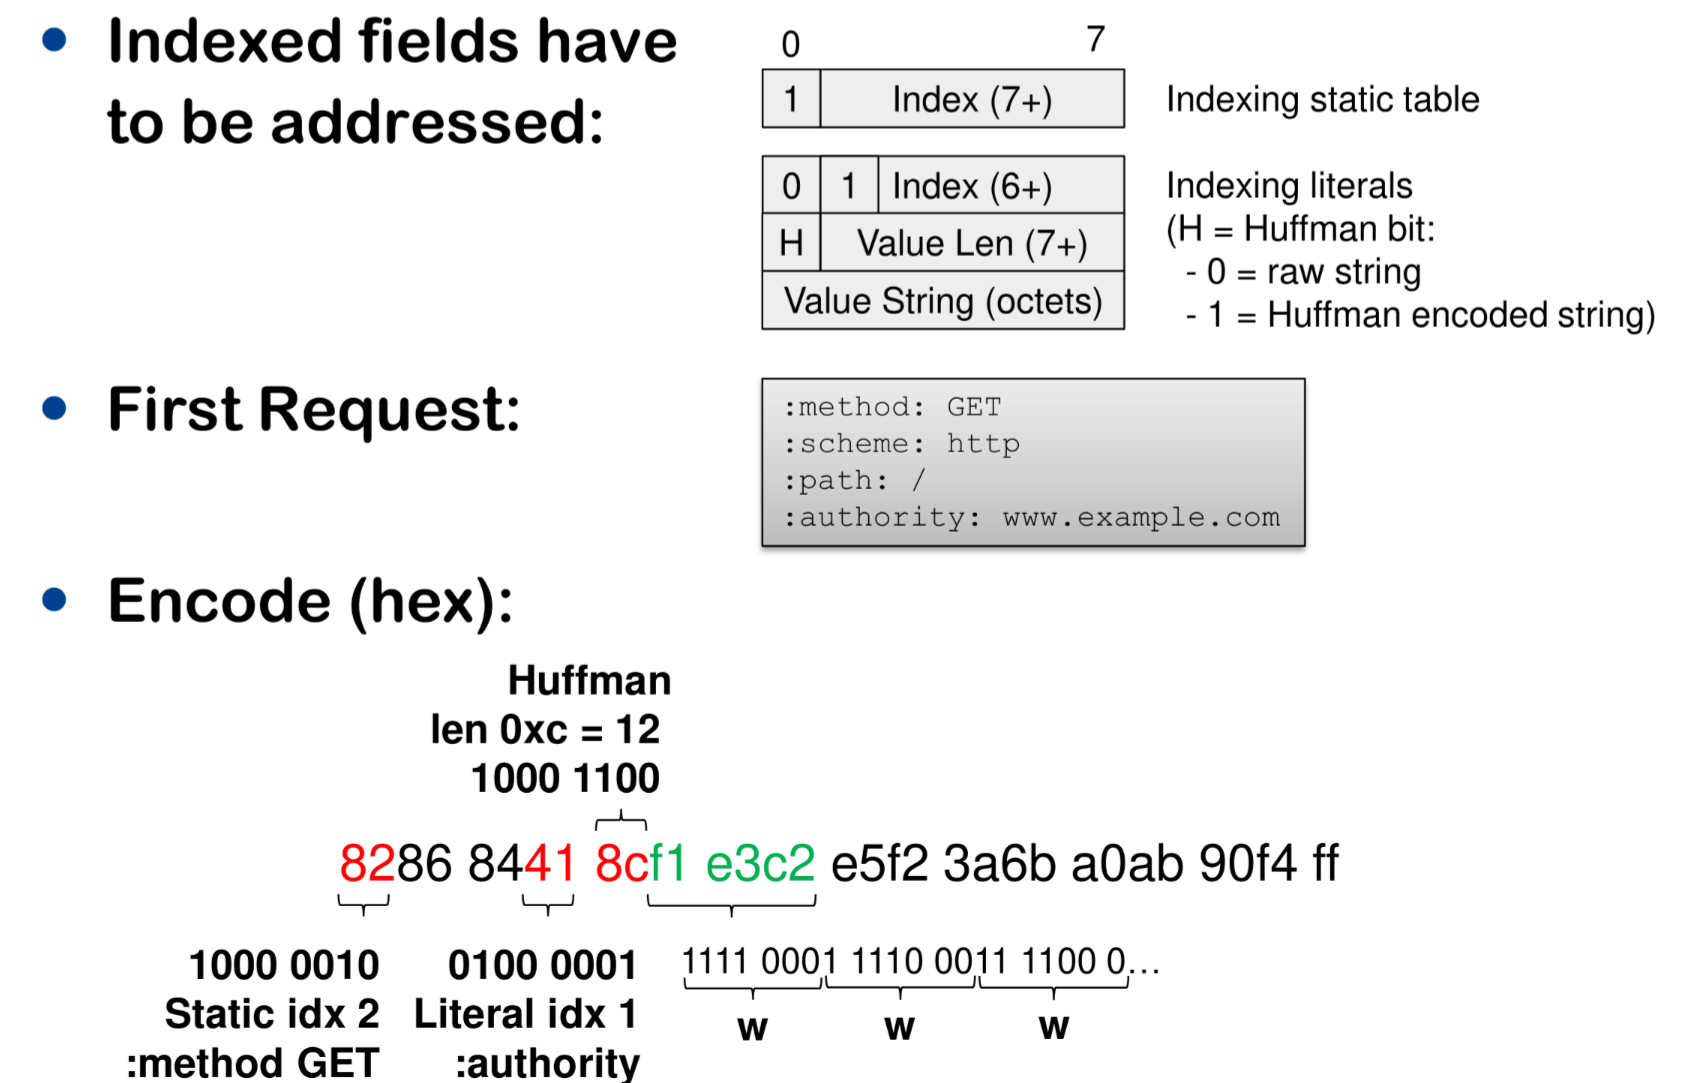
\includegraphics[width=\textwidth]{img/2-http2-huffman.png}
		\caption{Huffman encoding of HTTP/2 headers}
		\label{img-2-http2-huffman}
	\end{figure}	

	Unknown information can be learned and stored in the \textit{dynamic} part of the table.
	This way, the client can send shorter requests, saving bandwidth.
	Things to be learned start with \texttt{0b01XX}, as this signals, that the next bits are not Huffman encoded, but just plaintext.
	
	\paragraph{HTTP/2 and TLS}
	\label{pgf-http/2-and-tls}
	
	Both together build \texttt{HTTPS}, the secure version of HTTP.

	\vspace{0.5cm}
	\begin{alertbox}
		HTTP/3 is the newest version available for HTTP communication. 
	\end{alertbox}
	
	\subsection{Quick UDP Internet Connection (QUIC)}
	\label{ss-quick-udp-internet-connection-quic}

	QUIC uses many already established ideas and combines them into one single protocol, whilst avoiding the huge overhead introduced by TCP.

	Its main focus lies on better supporting HTTP, which it achieves by being able to map QUIC streams to HTTP/2 streams.
	
	\begin{figure}[H]
		\centering
		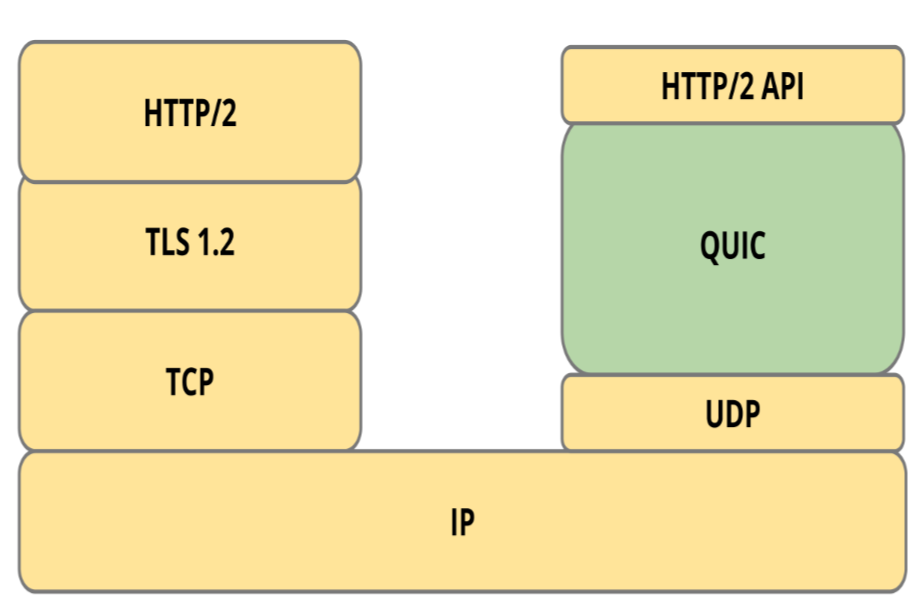
\includegraphics[width=0.6\textwidth]{img/2-quic-vs-http.png}
		\caption{Comparission of structure of QUIC and HTTP}
		\label{img-2-quic-vs-http}
	\end{figure}

	\paragraph{Multiplexing in QUIC}
	\label{pgf-multiplexing-in-quic}
	
	Because UDP is used instead of TCP, multiplexing is smoother, as Head-of-Line blocking is not possible anymore, due to missing control mechanismns in UDP.
	Of course, lost packets effect the stream the packet belonged to, but not all streams anymore.

	\paragraph{Connection Esablishment}
	\label{pgf-connection-esablishement}
	
	It uses the same idea as TCP fast open in \cref{tcp-fast-open}.
	Also TLS 1.3 is directly integrated in QUIC, which uses a 0-RTT design. 
	This allows to connect to servers, that you connected to in the past, by sending an old token, which proofs your identity.
	Of course there is a timeout, after which a completly new connection has to be established.

	Also, QUIC is not bound to the IP address of the parties, but to random 64-bit identifiers. 
	This allows for easier mobile usage.

	\begin{halfboxl}
		\begin{center}
			\begin{description}
				\item[CHLO] – Client Hellow
				\item[SNI] – Server Name Identification
				\item[CERT] – Certificate of Servers identity
				\item[REJ] – Reject
				\item[SHLO] – Server Hello
				\item[VER] - Verification
				\item[SRCT] – ?
			\end{description}
		\end{center}
	\end{halfboxl}%
	\begin{halfboxr}
		\vspace{-\baselineskip}
		\begin{figure}[H]
			\centering
			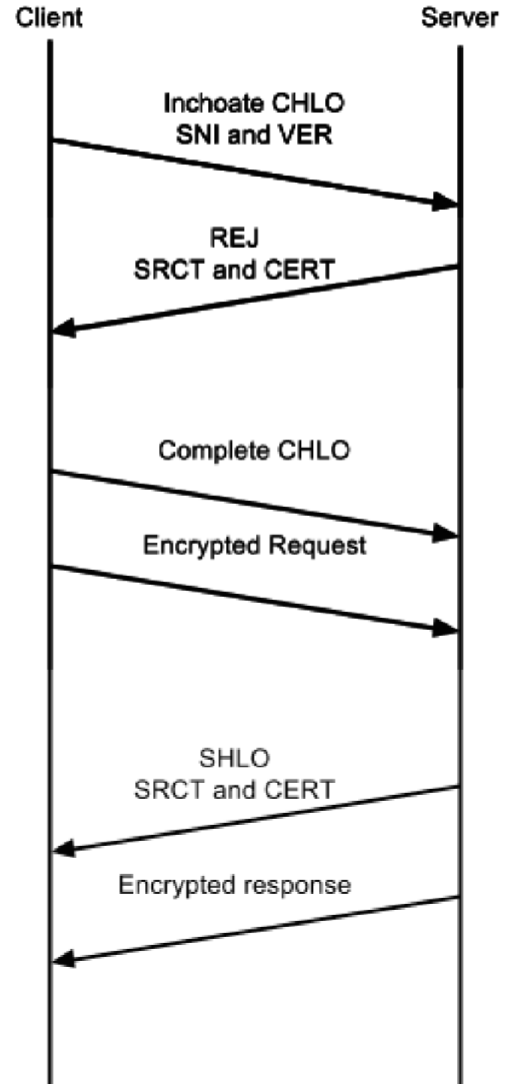
\includegraphics[width=0.3\textwidth]{img/2-quic-connecting.png}
			\caption{Connection to a server with QUIC}
			\label{img-2-quic-connecting}
		\end{figure}
	\end{halfboxr}

	Subsequent connections send header information, including verification and client hello, together with encrypted request.
	
	\paragraph{Congestion Control and Reliability in QUIC}
	\label{pgf-congestion-control-in-quic}
	
	Is based on TCP NewReno and also implements TCP Pacing, which spreads send packages evenly across RTT. 
	This avoids peaks, therefore lowering the risk of congesting the network.
	The reception of the first ACK (or NACK) is anticipated.

	Selective Acknowledgements are used. 
	Retransmissions have new sequence numbers, which increase monotonically.	

	\paragraph{Connection Migration}
	\label{pgf-connection-migration}
	
	Upon change of IP address of a client, TCP would drop the connection.
	QUIC is able to migrate the \enquote{new} connection into the old one, as connections are not identified by the clients ID, as explained in \cref{pgf-connection-esablishement}.
	
	\newpage
	\section{Kernel Networking}
	\label{s-kernel-networking}
	
	A kernel is used, to abstract the complete interaction with the hardware, s.t. user space programs do not need to worry about any of that.
	Basic kernel tasks include, but are not limited to:
	\begin{itemize}
		\item I/O interface for user space programs
		\item Handle interrupts
		\item Handle hardware utilization 
		\item Structuring hardware systems
		\item Virtualization
			\dots
	\end{itemize}

	No kernel ever trusts a user space program. 

	\begin{defi}{Kernel mode}
		The mode, that the kernel operates in. In kernel mode, software has full access of the hardware, and has priviledged rights.
	\end{defi}

	\begin{defi}{User mode}
		The mode, which user applications are assigned to. No hardware access, operations are only accepted, if kernel API is used.
	\end{defi}
	
	Kernel is not one single thread, instead utilizes threads for all common operations, which are spawned by a \texttt{init}-thread.

	\subsection{Interrupts}
	\label{ss-interrupts}
	
	Interrupts are flags set by hardware components to get the \enquote{attention} of the CPU.
	If an interrupt is raised, the current operation is paused immediately, unless the current operation itself is an interrupt handler.
	Interrupt handlers are functions within the kernel, that perform \textit{very} short actions, depending on what the interrupt is all about. 
	
	Interrupt sources (i.e. events, that cause an interrupt) can be system calls, external interrupt requests (by hardware), as well as exceptions.

	If an interrupt is called, a context change has to be performed, which introduces some computational overhead.

	\subsubsection{Interrupt Vectors and Handlers}
	\label{sss-interrupt-vectors}
	
	\begin{halfboxl}
		Might also be called \textit{Interrupt Descriptor Table (IDT)}.
		
		Interrupt vectors are used by the kernel to map a certain interrupt to the corresponding interrupt handler.
		This vector is a partition in the RAM, which maps interrupt sources to their respective handlers. 
		
		Interrupt handlers are loaded on boot, too. 
		Loading them on demand would lead to significant overhead, because everytime an interrupt would be raised, the correct handler has to be fetched from the hard  drive again.
		
		Some also important terminology:
		\begin{description}
			\item[PIC] Programmable Interrupt Controller
			\item[IRQ] Interrupt Request
		\end{description}
	\end{halfboxl}%
	\begin{halfboxr}
		\begin{figure}[H]
			\centering
			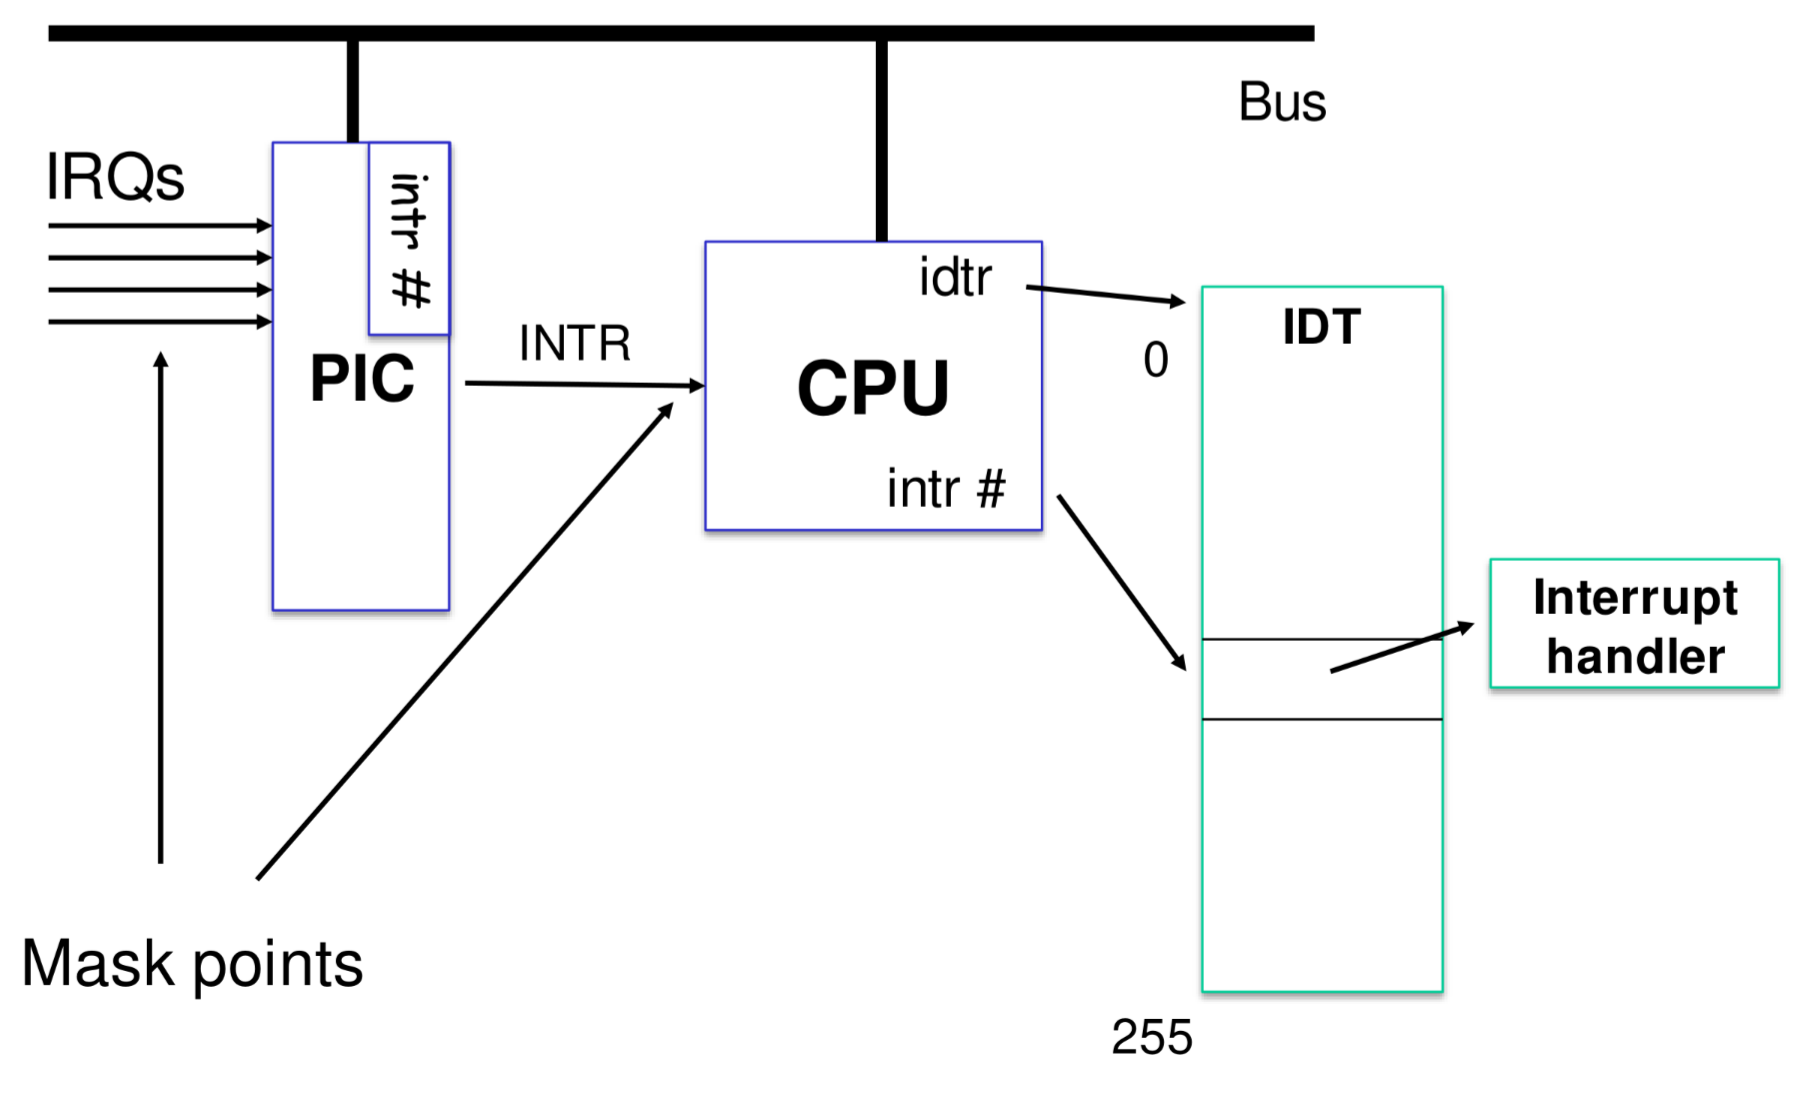
\includegraphics[width=\textwidth]{img/3-interrupt-handling-img.png}
			\caption{Conceptual scheme of how an interrupt is handled in \texttt{x86}}
			\label{img-3-interrupt-handling-img}
		\end{figure}
	\end{halfboxr}

	Interrupt handlers, under no circumstances, are not allowed to run for a long time or perform blocking operations, as the system gets unresponsive quickly.
	Often times, a flag is set, the actual handling of the interrupt is performed after a polling operation \cref{ss-polling}.
	
	\subsubsection{Context Switching}
	\label{sss-context-switching}
	
	When an interrupt is raised and the handler is called, the context, in which the previous process was running, has to be saved, in order to be able to continue the process after the interrupt was handled.

	This basically means storing register values to a structure in the kernel.

	In some cases, only a subset of registers is stored, as interrupts on that specific machine are not touching the other registers in any way. 
	This saves time, because unmodifiable data is not stored.

	\subsubsection{Interrupt Handling in Linux}
	\label{sss-interrupt-handling-in-linux}
	
	\alert{All the methods introduced in the following are executed in kernel space!}

	Handling of interrupts in Linux is twofold.
	
	\paragraph{Top Half}
	\label{pgf-top-half}
	
	This is the part that is executed on the spot.
	Those actions include:
	\begin{itemize}
		\item Mask other interrupts, block other interrupts from firing
		\item Save context of prev. process
		\item Call the proper interrupt handler and schedule it
	\end{itemize}

	\paragraph{Bottom Half}
	\label{pgf-bottom-half}
	
	This is where all the interesting stuff is happening.
	This is the \enquote{real} interrupt handler, which might be time critical, but nontheless is scheduled as a normal process, maybe with a higher priority.

	\begin{alertbox}
		Interrupt handlers cannot sleep. 
		This would be way to expensive.
		There also is no context to restore, as interrupt handlers are not normal functions. 
		It has no corresponding \textit{process control block}.
	\end{alertbox}
	
	\subsubsection{SoftIRQs}
	\label{sss-softirqs}
	
	\begin{defi}{SoftIRQ}
		A SoftIRQ is a process that gets scheduled with the highest possible priority. It does not interrupt the current process, but is certainely scheduled to be executed next.
	\end{defi}

	Those are statically allocated at boot. 
	A special struct is used to pass information to that SoftIRQ, which (not only) consits of:
	\begin{itemize}
		\item A pointer to the handler
		\item A pointer to the data that has to be passed to the SoftIRQ
	\end{itemize}

	These structures are used by \texttt{ksoftirqd}, the SoftIRQ daemon in the kernel, which spawns for every core of the CPU.

	A special function \fkt{do\_softirq} is used in order to call all pending SoftIRQs, they can also be called in response to a finished interrupt handler.
	These can be run on multiple cores simultaneously and \textbf{reschedule themselves}.

	It is strongly disregarded to implement SoftIRQs by yourself.

	\subsubsection{Tasklets}
	\label{sss-tasklets}
	
	An easier to use version is the \enquote{Tasklet}:

	\begin{defi}{Tasklet}
		Build on top of SoftIRQs, but can also be created dynamically.
		Tasklets are assigned to one concrete CPU, and are cache-affine.
	\end{defi}

	There are several functions to work with tasklets.
	\begin{itemize}
		\item \fkt{tasklet\_init} 
		\item \fkt{tasklet\_disable[\_nosync]} (\texttt{*\_nosync} does not wait for the tasklet to return) 
		\item \fkt{tasklet\_kill}
	\end{itemize}
	
	\textbf{Note:} Tasklets are run in interrupt context.

	\subsubsection{Work Queues}
	\label{sss-work-queues}
	
	Is a subsystem of the Linux kernel. There is one dedicated \textit{default worker thread} per CPU.
	You could also create your own \textit{special worker threads}. 
	Often times, this is not needed.
	However, if you need to perform much processing, defer to a worker thread in order to be able to handle incoming packets directly, when they are handed to your main thread.

	Work executed in the default worker thread should ideally not block, as this prevents other tasks to be completed.

	\subsubsection{Overview and Comparisson}
	\label{sss-overview}
	
	\begin{figure}[H]
		\centering
		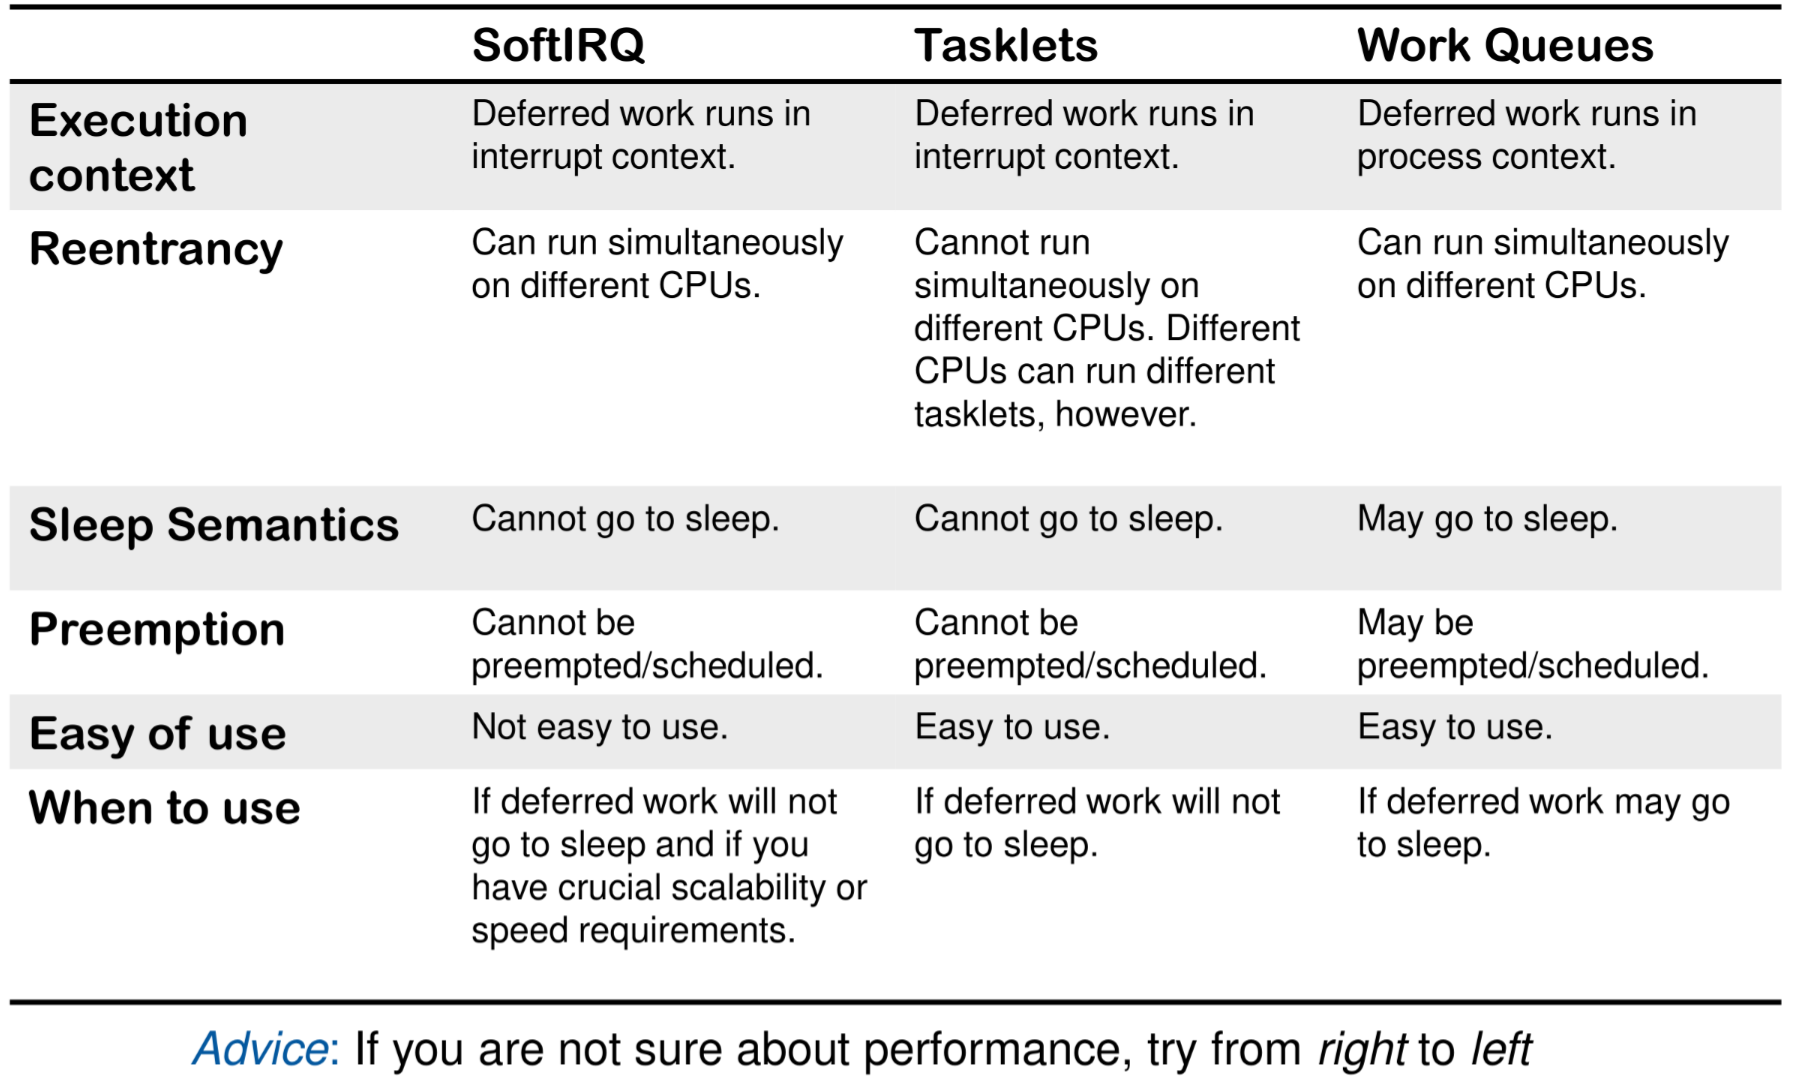
\includegraphics[width=\textwidth]{img/3-softirq-vs-rest.png}
		\caption{Comparisson of the three introduced methods}
		\label{img-3-softirq-vs-rest}
	\end{figure}

	\subsection{Polling}
	\label{ss-polling}
	
	Polling is constant, periodical checking, if a certain condidtion is met or a flag is set.
	The polling period is critical, as too fast checking may overload the CPU, whereas too slow checking leads to not being able to handle fast occuring events.

	\subsection{Handling Pakets in the Kernel}
	\label{ss-handling-pakets-in-the-kernel}
	
	A packet follows the depicted path below.

	\begin{figure}[H]
		\centering
		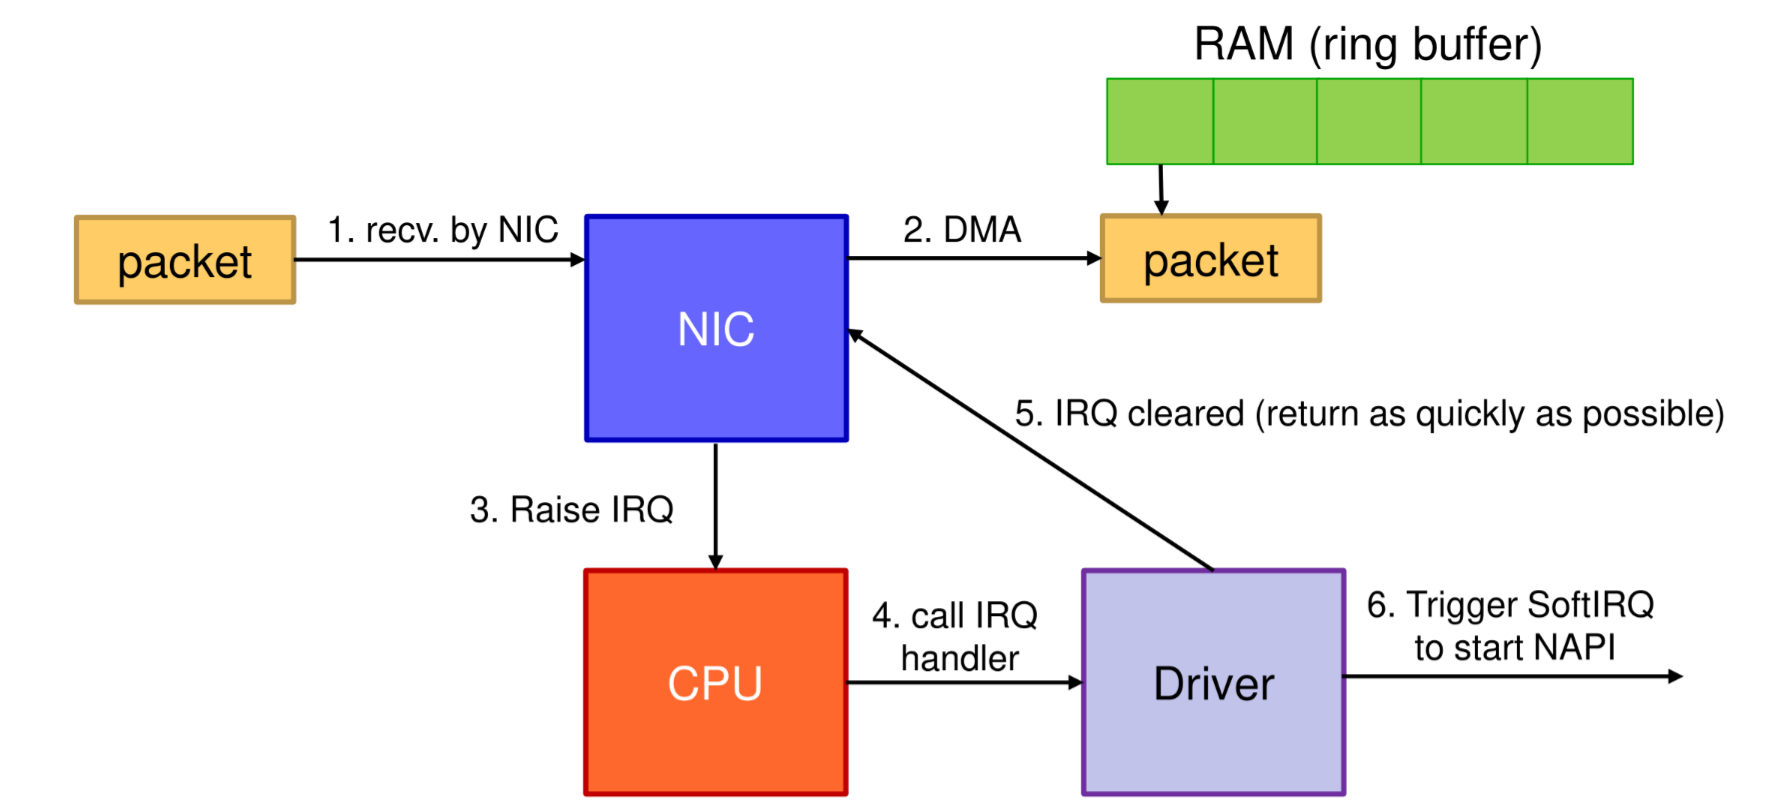
\includegraphics[width=\textwidth]{img/3-packets-kernel.png}
		\caption{Processing of a packet}
		\label{img-3-packets-kernel}
	\end{figure}

	The SoftIRQ in (6.) is marked pending, and then is executed from the kernel daemon responsible for SoftIRQs, \texttt{ksoftirqd}. This SoftIRQ calls \fkt{net\_rx\_action}, which disables NIC interrupts, and starts a polling mechanism, see \cref{img-3-napi}.
	This is done to efficiently receive data without being interrupted.

	\begin{figure}[H]
		\centering
		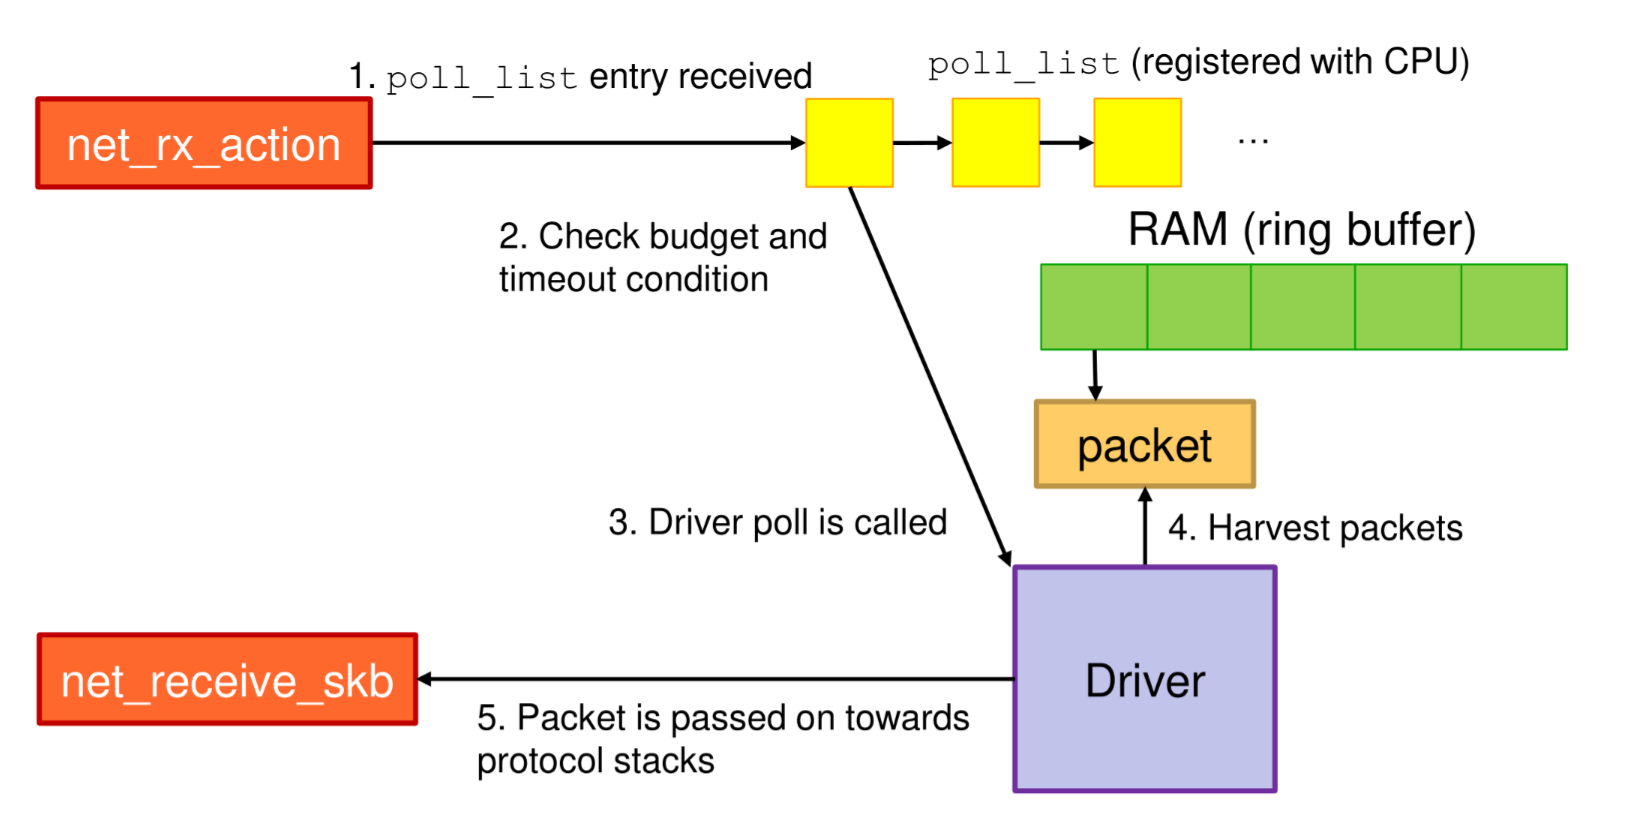
\includegraphics[width=\textwidth]{img/3-napi.png}
		\caption{Inner workings of the New API}
		\label{img-3-napi}
	\end{figure}

	The budget in step (2.) prevents the poll to hug all system resources, as with each handled packet, the counter of the budget is decreased by one.	
	This enables efficient handling of bursts, without consuming the whole CPU for a long time, if there were much more packets to come.

	When a concrete packet is processed, the corresponding memory in the RAM is un-mapped, s.t. the network driver cannot write to that specific location anymore. This way, packets can be processed in-place.

	After a packet is processed, the memory is re-mapped.

	\subsection{Socket Buffers}
	\label{ss-socket-buffers}
	
	These are the most fundamental parts of networking.

	\begin{figure}[H]
		\centering
		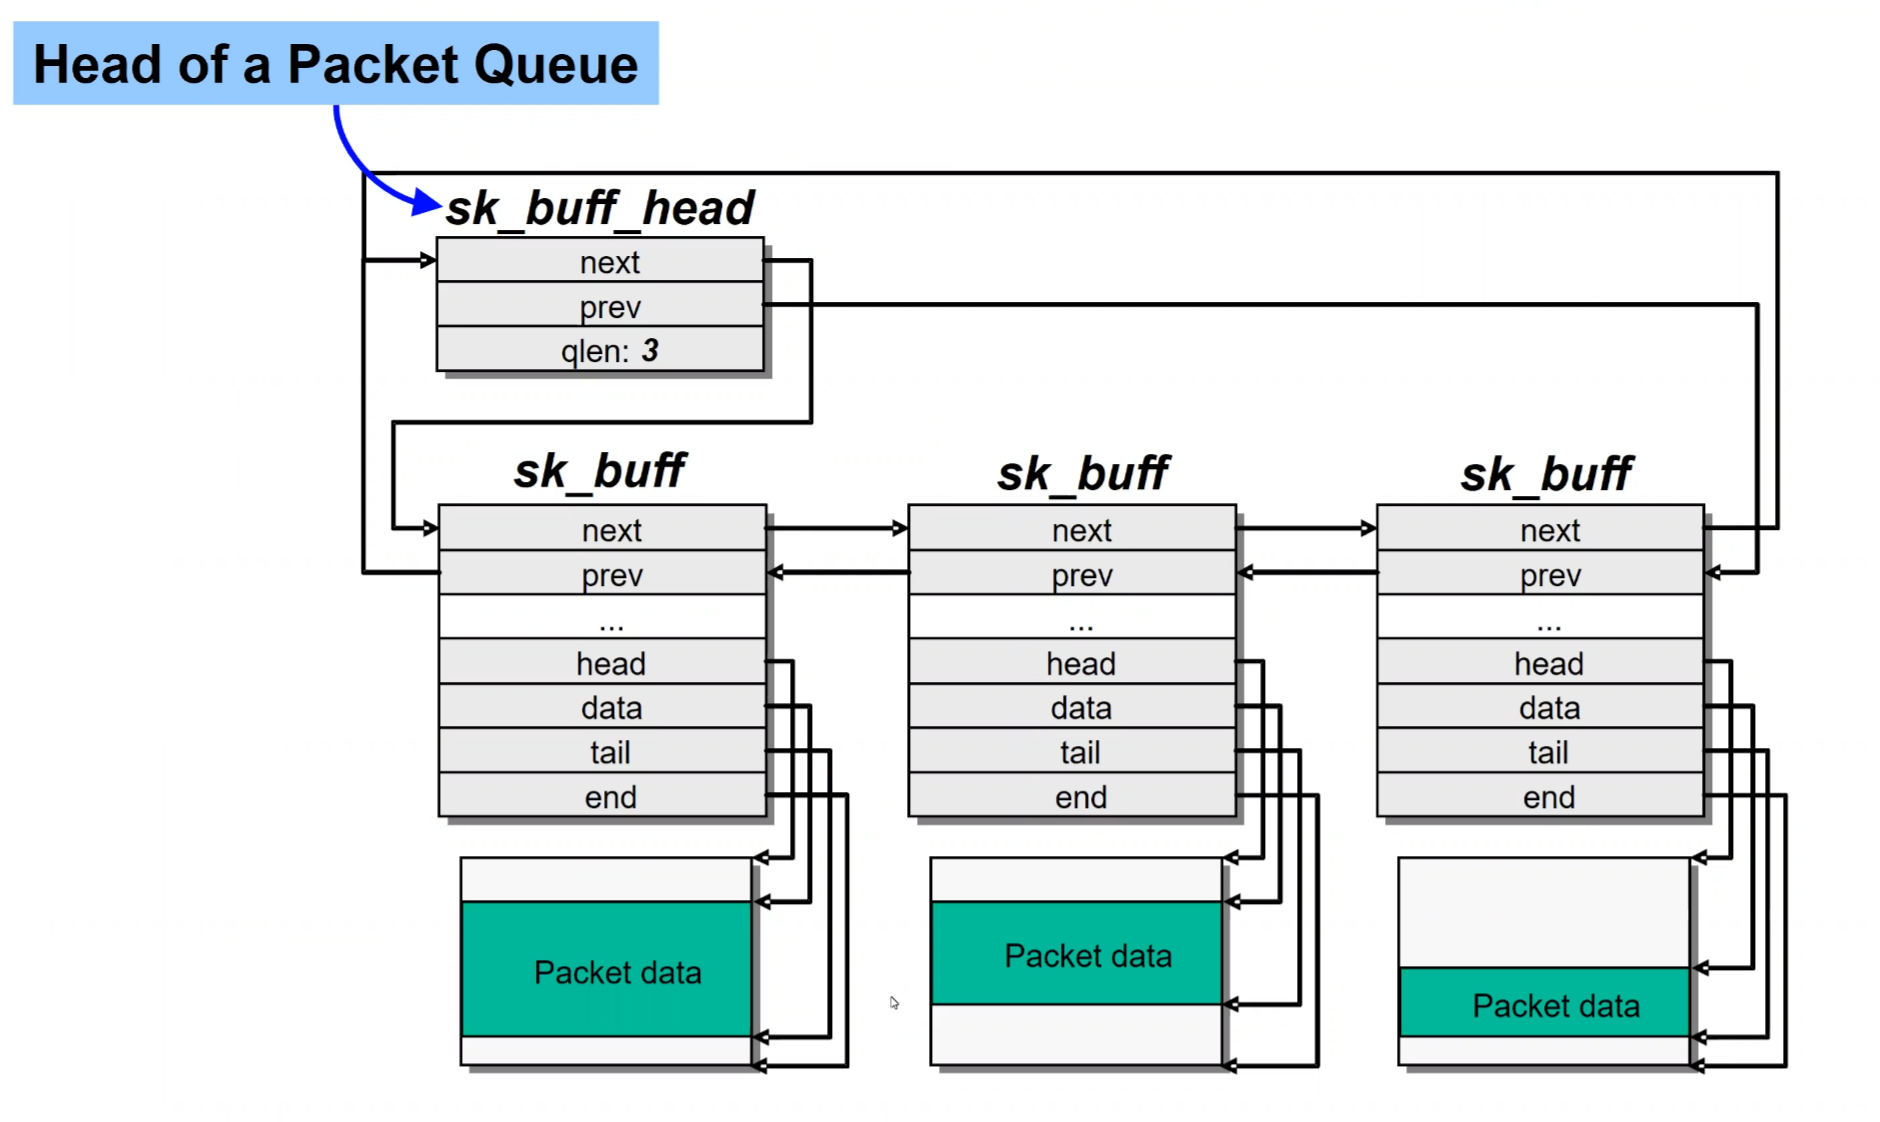
\includegraphics[width=\textwidth]{img/3-skbuff.png}
		\caption{Depiction of usage of \texttt{sk\_buff}}
		\label{img-3-skbuff}
	\end{figure}

	Each \texttt{sk\_buff} is a double linked list.
	The position of the start of each header (TCP, UDP, IP, whatever) is stored in data fields within \texttt{sk\_buff}.
	There are also field to store pointers to headers within headers (\texttt{*\_inner\_*}).
	Some important components:
	\begin{description}
		\item[\texttt{next}] for double linked list
		\item[\texttt{prev}] for double linked list
		\item[\texttt{list}] to what list the buffer belongs
		\item[\texttt{sk}] socket that packet belongs to
		\item[\texttt{dev}] device the packet belongs to
		\item[\texttt{stamp}] timestamp
		\item[\texttt{sc}] security path traversed in the packet
		\item[\texttt{cb}] control block, used for flags
		\item[\texttt{len}] total length of packet
		\item[\texttt{data\_len}] lenght of payload
		\item[\texttt{user}] reference counter
		\item[Header information] as described in the paragraph above
	\end{description}
	
	\subsubsection{Working on Data with \texttt{sk\_buff}s}
	\label{sss-working-on-data-with-sk_buffs}
	
	
	\begin{halfboxl}
		There exist blocks of memory resevered by the kernel, which are able to hold a complete packet, including header information.
		These are \textit{only} used by the kernel.

		Note, that the data pointer starts on top of the IP header. 
		This is, because, the most upper layer (MAC) is not interessted in where the actual payload starts. 
		It just needs to know, where the data starts, that needs to be send.

		On reception of such a packet, the headers have information needed to disassemble the whole packet into different headers and finally the payload, by providing a field which points to the start of the data, as viewed for that protocol. 
		For example, the IP header might have a length field, that when added to the address of the IP header, points to the start of the UDP header.
	\end{halfboxl}%
	\begin{halfboxr}
		\vspace{-\baselineskip}
		\begin{figure}[H]
			\centering
			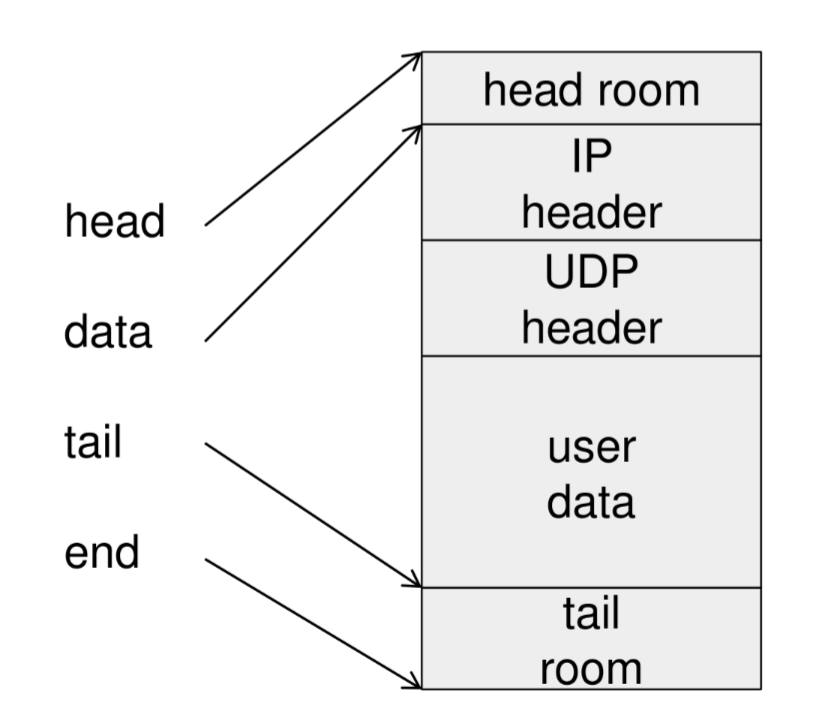
\includegraphics[width=\textwidth]{img/3-data-skbuff.png}
			\caption{Data representation in an \texttt{sk\_buff}}
			\label{img-3-data-skbuff}
		\end{figure}
	\end{halfboxr}
	
	\subsection{Packet Processing Workflow}
	\label{ss-protocol-processing-workflow}
	
	\fkt{netif\_receive\_skb} in \cref{img-3-packet-processing-workflow} is called by a function somewhere in \fkt{net\_receive\_skb} form \cref{img-3-napi}.

	\begin{figure}[H]
		\centering
		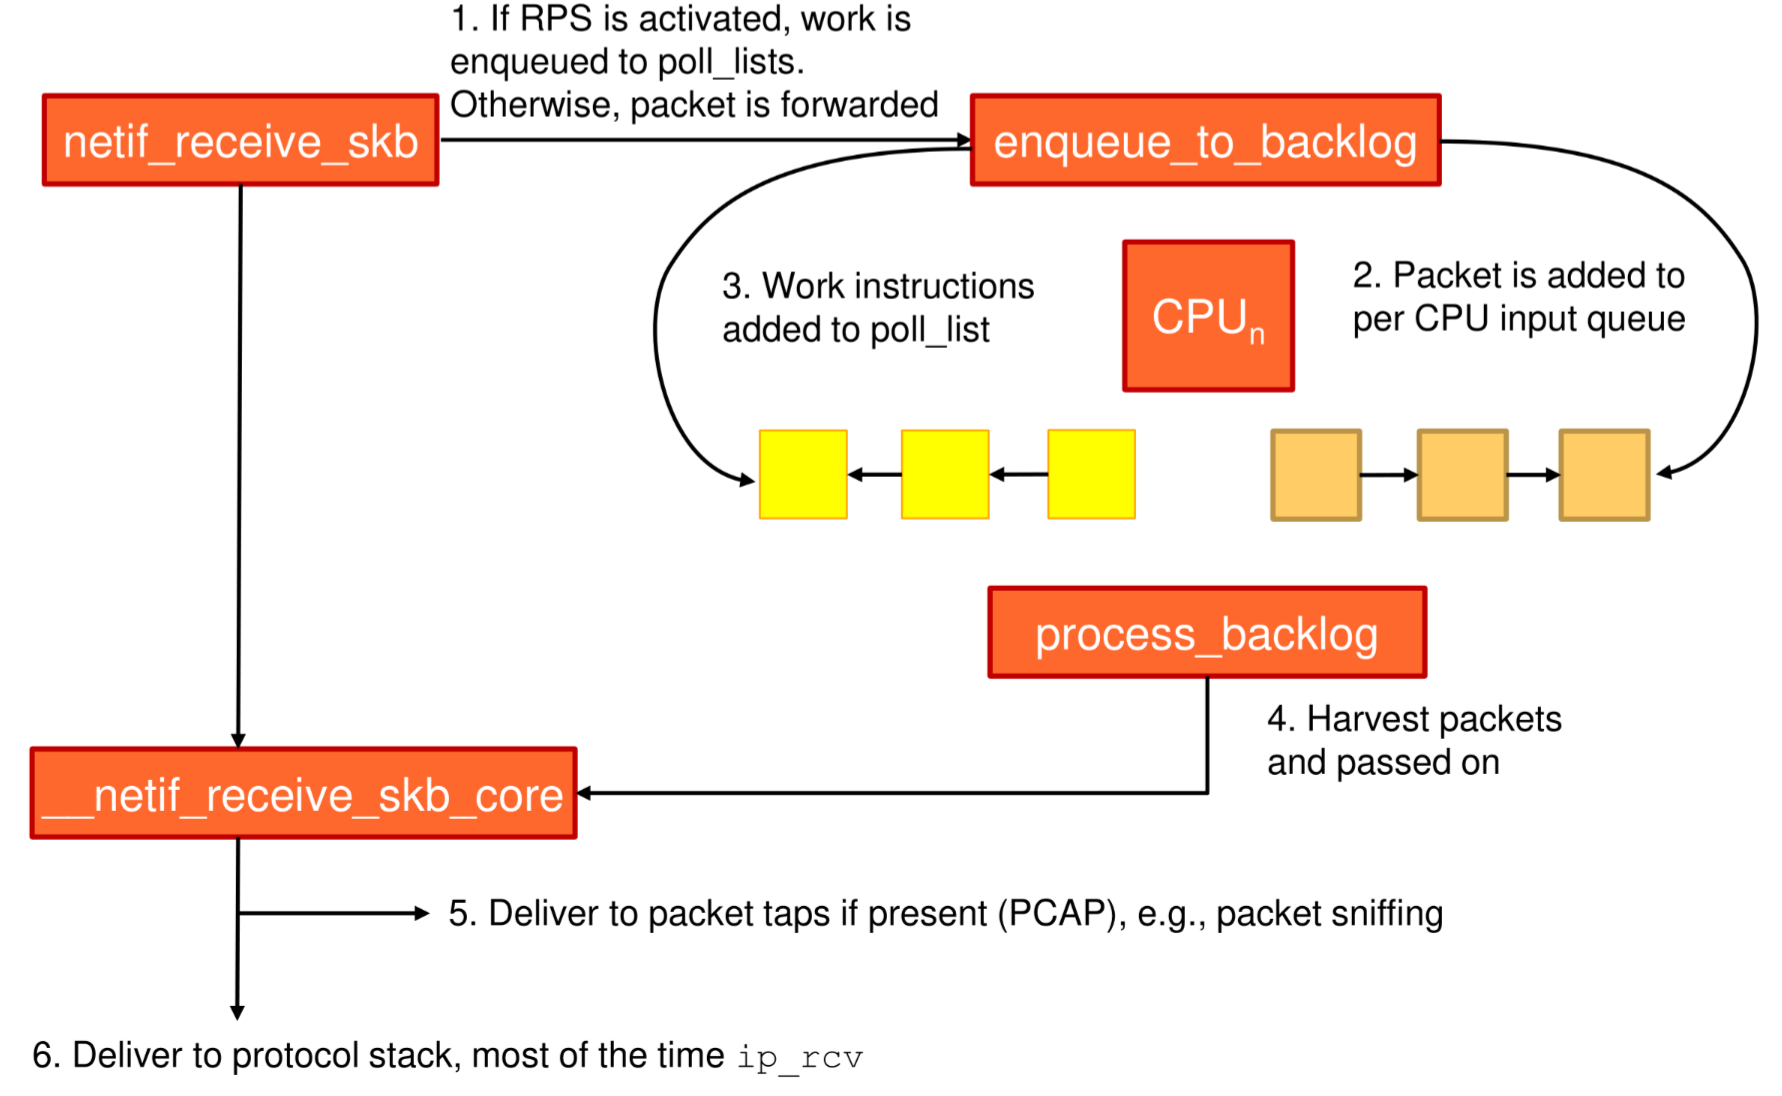
\includegraphics[width=0.85\textwidth]{img/3-packet-processing-workflow.png}
		\caption{Packet processing workflow}
		\label{img-3-packet-processing-workflow}
	\end{figure}
	
		
	





	

	
				






















\end{document}
